\documentclass[11pt]{article}
\usepackage[T1]{fontenc}
\usepackage{lmodern}
\usepackage[margin=1in]{geometry}
\usepackage{amsmath,amssymb,amsthm,mathtools}
\usepackage{microtype}
\usepackage{enumitem}
\usepackage{graphicx,placeins}
\usepackage{tikz}
\usetikzlibrary{arrows.meta,positioning,shapes.geometric,fit}
\usepackage{xcolor}
\definecolor{linkblue}{RGB}{26,65,110}
\usepackage[colorlinks=true,linkcolor=linkblue,citecolor=linkblue,urlcolor=linkblue]{hyperref}
\usepackage[nameinlink,capitalise,noabbrev]{cleveref}
\hypersetup{pdftitle={Commuting Division-Coefficient Forms and the Artinian Eisenbud--Green--Harris Conjecture},pdfauthor={OpenAI},pdfsubject={Hilbert functions and central division algebras}}
\pdfinfoomitdate=1
\pdftrailerid{}
\pdfsuppressptexinfo=15
\setlength{\emergencystretch}{2em}
\setlist{itemsep=3pt,topsep=5pt}
\newtheorem{theorem}{Theorem}[section]
\newtheorem{proposition}[theorem]{Proposition}
\newtheorem{lemma}[theorem]{Lemma}
\newtheorem{corollary}[theorem]{Corollary}
\theoremstyle{definition}
\newtheorem{definition}[theorem]{Definition}
\newtheorem{notation}[theorem]{Notation}
\theoremstyle{remark}
\newtheorem{remark}[theorem]{Remark}
\numberwithin{equation}{section}
\newcommand{\C}{\mathbb C}
\newcommand{\Z}{\mathbb Z}
\newcommand{\Q}{\mathbb Q}
\newcommand{\R}{\mathbb R}
\newcommand{\PP}{\mathbb P}
\newcommand{\A}{\mathbb A}
\newcommand{\cO}{\mathcal O}
\newcommand{\cH}{\mathcal H}
\newcommand{\cL}{\mathcal L}
\newcommand{\cF}{\mathcal F}
\newcommand{\cE}{\mathcal E}
\newcommand{\cD}{\mathcal D}
\newcommand{\sm}{\mathrm{sm}}
\DeclareMathOperator{\Spec}{Spec}
\DeclareMathOperator{\Proj}{Proj}
\DeclareMathOperator{\Sym}{Sym}
\DeclareMathOperator{\Pic}{Pic}
\DeclareMathOperator{\End}{End}
\DeclareMathOperator{\Hom}{Hom}
\DeclareMathOperator{\Hilb}{Hilb}
\DeclareMathOperator{\ch}{ch}
\DeclareMathOperator{\td}{td}
\DeclareMathOperator{\rk}{rk}
\DeclareMathOperator{\Gal}{Gal}
\DeclareMathOperator{\coker}{coker}
\DeclareMathOperator{\im}{im}
\title{Commuting Division-Coefficient Forms and the Artinian Eisenbud--Green--Harris Conjecture}
\author{OpenAI}
\date{September 23, 2026}
\begin{document}
\maketitle
\begin{abstract}
We prove the Eisenbud--Green--Harris conjecture over every characteristic-zero
field for homogeneous regular sequences of any positive length, with degrees
at least two. Thus every homogeneous ideal containing such a sequence has the
Hilbert function of a monomial ideal containing the corresponding pure powers.
\end{abstract}
\clearpage
\begingroup
\small
\tableofcontents
\endgroup
\clearpage
\section{Introduction}\label{sec:introduction}

A homogeneous ideal is constrained both by the equations it contains and by the dimensions of its graded pieces. The Eisenbud--Green--Harris conjecture predicts a particularly concrete form for this constraint: a regular sequence can be replaced by the corresponding pure powers without changing the Hilbert function of a containing ideal. We prove this assertion over the complex numbers in its Artinian formulation, for arbitrary degrees, and then deduce the full characteristic-zero statement for regular sequences of arbitrary positive length. The main construction provides more than the Hilbert-function comparison: it replaces the polynomial variables by commuting linear forms with division-algebra coefficients and retains an ordered basis of the entire polynomial algebra.

Let $S=\C[x_1,\ldots,x_n]$ with its standard grading. For a homogeneous ideal $I\subseteq S$, write
\[
 H_{S/I}(d)=\dim_\C(S/I)_d\qquad(d\ge0).
\]
A sequence $f_1,\ldots,f_n$ of positive-degree homogeneous elements is \emph{regular} if multiplication by $f_i$ is injective on $S/(f_1,\ldots,f_{i-1})$ for each $i$. Its quotient has Hilbert series
\[
 \Hilb_{S/(f_1,\ldots,f_n)}(t)
 =\prod_{i=1}^n(1+t+\cdots+t^{a_i-1}),\qquad a_i=\deg f_i,
\]
so every ideal containing it has an Artinian quotient.

Eisenbud, Green, and Harris arrived at the conjecture through extensions
of Castelnuovo theory. Section~4 of \cite{EGH93} formulates the quadratic
case and then proposes the arbitrary-degree pure-power comparison.
Their Cayley--Bacharach interpretation already appears in
\cite[Section~3]{EGH93} and is developed further in
\cite[Section~2.1]{EGH96}. The pure-power model turns the geometric
constraints into a problem about monomials with bounded exponents.
The construction below supplies that model for an arbitrary homogeneous
regular sequence.

We first state this construction. If $k/\C$ is a field extension and
$\Delta$ is a central division $k$-algebra, then
$\Delta[x_1,\ldots,x_n]$ denotes the polynomial algebra with central
variables $x_j$. The coefficients in $\Delta$ have degree zero. A
collection of its linear forms may commute even when their individual
coefficients do not.

\begin{theorem}[Commuting-form construction]\label{thm:construction}
Let $n\ge1$, let $2\le a_1\le\cdots\le a_n$, and let
$f_1,\ldots,f_n$ be a homogeneous regular sequence in
$\C[x_1,\ldots,x_n]$ with $\deg f_i=a_i$. There exist a finitely
generated field extension $k/\C$, a finite-dimensional central division
$k$-algebra $\Delta$, and a commutative graded $k$-subalgebra
\[
 k[x_1,\ldots,x_n]\subseteq A\subseteq\Delta[x_1,\ldots,x_n]
\]
generated by finitely many pairwise commuting linear forms, with
distinguished $t_1,\ldots,t_n\in A_1$, such that
\begin{equation}\label{eq:construction-triangular}
 t_i^{a_i}=c_i f_i+\sum_{l<i}B_{il}f_l+\sum_{d>i}C_{id}t_d
 \qquad(1\le i\le n).
\end{equation}
Here $c_i\in k^\times$, $B_{il}\in A_{a_i-a_l}$, and
$C_{id}\in A_{a_i-1}$. Moreover, $A$ is finite over $k[x]$, and
\[
 \{t_1^{\alpha_1}\cdots t_n^{\alpha_n}:
             \alpha\in\Z_{\ge0}^n\}
\]
is a basis of the full polynomial algebra $\Delta[x]$ as a left
$\Delta$-vector space.
\end{theorem}

The basis is not restricted to the complete-intersection quotient. In
particular, it describes every graded piece before any additional ideal
is imposed. This is the interface used for resolution transfer in the
companion paper \cite[Lemma~4.1]{BettiCompanion}.
For Hilbert functions, a least-exponent argument already gives the
following consequence.

\begin{corollary}[Artinian Eisenbud--Green--Harris]\label{thm:main}
Let $n\ge1$ and $2\le a_1\le\cdots\le a_n$. Suppose that a homogeneous ideal $I\subseteq\C[x_1,\ldots,x_n]$ contains a regular sequence $f_1,\ldots,f_n$ with $\deg f_i=a_i$. There is a monomial ideal $J\subseteq\C[x_1,\ldots,x_n]$ such that
\[
 x_i^{a_i}\in J\quad(1\le i\le n),
 \qquad
 H_{S/J}(d)=H_{S/I}(d)\quad\text{for every }d\ge0.
\]
\end{corollary}

Thus the Artinian Eisenbud--Green--Harris conjecture is resolved positively over $\C$. One ideal $J$ realizes the entire Hilbert function, and there is no restriction on the further generators of $I$.

To describe the lex-plus-powers formulation, order variables by
$x_1>\cdots>x_n$, and let $J$ be the monomial ideal in the corollary.
In degree $d$, among monomials outside
$P=(x_1^{a_1},\ldots,x_n^{a_n})$, take the
$q_d=\dim_\C J_d-\dim_\C P_d$ lexicographically largest ones. The
Clements--Lindstr\"om theorem says that these degreewise choices, together
with $P$, form an ideal whenever the Hilbert function comes from an ideal
containing $P$ \cite{CL69}. Thus Corollary~\ref{thm:main} also gives one
lex-plus-powers ideal with the entire prescribed Hilbert function. We use
the exact compression statement in
\cite[Theorem~2.1(i)]{CDS22}; it is not a premise of
Theorem~\ref{thm:construction}.

The Hilbert-function conclusion is not restricted to Artinian quotients
or to the coefficient field \(\C\).

\begin{corollary}[Eisenbud--Green--Harris in characteristic zero]
\label{cor:characteristic-zero}
Let \(F\) be a field of characteristic zero, let
\(S_F=F[x_1,\ldots,x_n]\) be standard graded, and let
\[
 1\le c\le n,\qquad 2\le a_1\le\cdots\le a_c.
\]
If a homogeneous ideal \(I\subseteq S_F\) contains a homogeneous regular
sequence \(f_1,\ldots,f_c\) with \(\deg f_i=a_i\), there is a monomial ideal
\(J\subseteq S_F\) containing
\(P_F=(x_1^{a_1},\ldots,x_c^{a_c})\) such that
\[
 \dim_F(S_F/J)_d=\dim_F(S_F/I)_d\qquad(d\ge0).
\]
Moreover, \(J\) may be chosen lex-plus-powers: in each degree its monomials
outside \(P_F\) are the lexicographically greatest
\(\dim_F I_d-\dim_F(P_F)_d\) monomials outside \(P_F\), for the order
\(x_1>\cdots>x_n\).
\end{corollary}

The proof in Section~\ref{subsec:generality} combines the Artinian result
with a reduction to full regular sequences and descent through a finitely
generated coefficient field. The division-algebra construction of
Theorem~\ref{thm:construction} itself concerns full regular sequences over
\(\C\). Section~\ref{sec:consequences} also gives local-cohomology
inequalities for the resulting lex-plus-powers ideal and a
scheme-theoretic quadratic Cayley--Bacharach bound.

\subsection{Earlier results on EGH}

Results depending only on the degrees of the regular sequence have
covered important ranges. Caviglia and Maclagan proved EGH when
$a_i>\sum_{j<i}(a_j-1)$ for $i\ge3$ \cite{CM08}; Caviglia and De Stefani
extended this to the non-strict inequalities
\cite[Theorem~A]{CDeS20}. For quadratic sequences, Chen proved the case
of at most four variables \cite[Theorem~2.2]{Chen12}. Caviglia,
De Stefani, and Sbarra give an independent proof for five quadrics,
alongside a systematic account of the conjecture
\cite[Theorem~4.14]{CDS22}.

Other results use additional structure of the forms or the containing
ideal. Abedelfatah proves EGH when all forms of the regular sequence
split into linear factors \cite[Corollary~4.3]{Abedelfatah15}.
Cooper treats subsets of finite reduced complete intersections of
types $(a,b)$, $(2,a,b)$, and $(3,a,a)$ \cite{Cooper12}.
Chong uses liaison to treat sequentially bounded licci ideals with a
minimal first link and a minimally contained regular sequence; his
results include height-three Gorenstein ideals under the corresponding
minimal-containment condition
\cite[Theorem~3 and Corollary~11]{Chong16}.

Recent work addresses both small-degree cases and asymptotic ranges.
Abedelfatah proves EGH for quadratic almost complete intersections in
six variables \cite[Theorem~4.3]{Abedelfatah26}. Kuzmanovski obtains
Hilbert-function comparisons through prescribed degree ranges when the
initial degree is sufficiently large
\cite[Theorems~1.4--1.5]{Kuzmanovski26}. The construction here applies to
arbitrary regular sequences of the stated degrees and gives one ideal
with the same Hilbert function in every degree.

\subsection{Proof strategy and its methods}

The triangular identities in Theorem~\ref{thm:construction} make the
\(t_i\) a regular system of parameters on the finite module
\(\Delta[x]\) over \(A\). Since they have degree one, a Hilbert-series
count gives the full ordered basis. Least exponents of elements of an
extended ideal then form one upward-closed set, defining the ordinary
monomial ideal. Section~\ref{sec:reduction} establishes this algebraic
reduction before the construction begins.

We construct the rows from \(i=n\) down to \(i=1\). At a stage with
\(b=a_i\), the aim is to express a suitable right-hand side of the new
row as a sum \(\ell_1^b+\cdots+\ell_M^b\) of powers of existing forms,
then combine these powers two at a time until the sum becomes \(t_i^b\).
Two difficulties govern the construction: the binary addition matrices
must have coefficients in a division algebra containing the old
coefficients, and the earlier power identities must remain available
when the next degree is smaller.

To retain those identities, we use a finite-dimensional space \(U\)
of formal linear forms containing the variables \(x_j\) and the forms
\(t_d\) already constructed, together with an ideal
\(Q\subseteq\Sym U\) generated in degrees one and two. Evaluation
recovers the actual commuting forms, and every earlier identity holds
modulo \(Q\). Let \(\mathfrak j_b\) be the degree-\(b\) part of
\[
 (Q,f_1,\ldots,f_i,t_{i+1},\ldots,t_n)\subseteq\Sym U.
\]
A linear functional \(\lambda\) on \(\Sym^b U\) that annihilates
\(\mathfrak j_b\) defines the
degree-\(b\) polynomial \(w_\lambda(\ell)=\lambda(\ell^b)\) on \(U\).
If \(W\) is their space, then
\[
 \sum_{m=1}^M\ell_m^b\in\mathfrak j_b
 \quad\Longleftrightarrow\quad
 \sum_{m=1}^M w(\ell_m)=0\qquad(w\in W).
\]
Let \(X\subseteq\PP(U^{\oplus M})\) be the projectivization of the
common zero set of these equations.

The geometric safeguard is that the projective zero set of \(Q\)
contains no curve of bounded small degree. Section~\ref{sec:low-relations}
constructs such data from independent quadratic equations, proves that
finite homogeneous enlargement preserves the property, and uses it to
show that every nonzero \(w\in W\) has an irreducible factor of
multiplicity one. For sufficiently many blocks, Section~\ref{sec:parameters}
then proves that \(X\) is an integral
complete intersection and that the nonzero cone over its smooth locus
has arbitrarily high connectivity. The argument allows nonisolated
singularities and requires only one simple factor in each member of
\(W\).

The binary addition matrices come from a curve with three sections
satisfying \(z^b=u^b+v^b\). A generic degree-zero line bundle makes
multiplication by these sections linear in \(u,v\). This use of matrix
pencils belongs to the generalized Clifford-algebra and vector-bundle
correspondence developed by van den Bergh \cite{VanDenBergh87} and
Kulkarni \cite{Kulkarni03}; the trivial finite-pushforward formulation
appears in \cite[Proposition~2.5]{CKM12}.
Section~\ref{sec:curves} constructs the required curve and pencils
explicitly, together with a finite group action. A matrix representation
alone does not make the coefficient algebra division.

The two Picard varieties of the curve serve different purposes:
degree-zero line bundles parametrize the matrices, while the
degree-one Picard variety supplies a free group action and maps carrying
prescribed characters. Equivariant descent first gives a central simple
algebra. To prove that it is division, we show that the dimension of
every finite right module is divisible by the dimension of the algebra,
both measured over its center. A nonzero proper right ideal would
contradict this divisibility.

Section~\ref{sec:descent} uses a determinant-of-cohomology
correction to relate module dimensions to Euler characteristics on a
product of Picard varieties. The free action also gives divisibility
of Euler characteristics for the corresponding family over \(X\),
after twisting by \(\cO_X(l)\). The correction uses the formalism of
Knudsen and Mumford
\cite{KnudsenMumford76}, and its numerical effect follows from
Grothendieck's Riemann--Roch theorem \cite{BorelSerre58}.
Section~\ref{sec:index} uses the character maps, connectivity of the
smooth cone, and integral topological \(K\)-theory to compare these
Euler characteristics and prove that the algebra is division while
retaining the old coefficient algebra.

The use of highly connected algebraic parameter spaces and finite
quotients is related to the Godeaux--Serre approximation method
\cite[Section~5]{Totaro99}. Topological restrictions on an algebraic
index have a close precedent in
Antieau and Williams \cite[Theorem~3.4]{AntieauWilliams13}.
Here the determinant correction and integral \(K\)-theory pushforward
separate divisibility by the new group order from divisibility by the
old algebra's degree. Consequently the required connectivity can be
fixed before enlarging the number of summands. Finally,
Section~\ref{sec:assembly} verifies the characters that make the new
output invariant and retains the new row through a finite extension
defined by linear and quadratic relations. This closes the induction.

When every $a_i=2$, Corollary~\ref{thm:main} gives the quadratic assertion.
The complete-intersection Hilbert series is then $(1+t)^n$, and the
standard monomials of a monomial ideal containing $x_1^2,\ldots,x_n^2$
correspond to a family of subsets of $\{1,\ldots,n\}$ closed under
taking subsets. Here this
special case follows from the same ordered-basis construction as all
other degree sequences; no separate quadratic theorem is required.

Figure~\ref{fig:construction} records the dependencies within one induction
step and the return to its hypotheses before the next row.

\begin{figure}[!htbp]
\centering
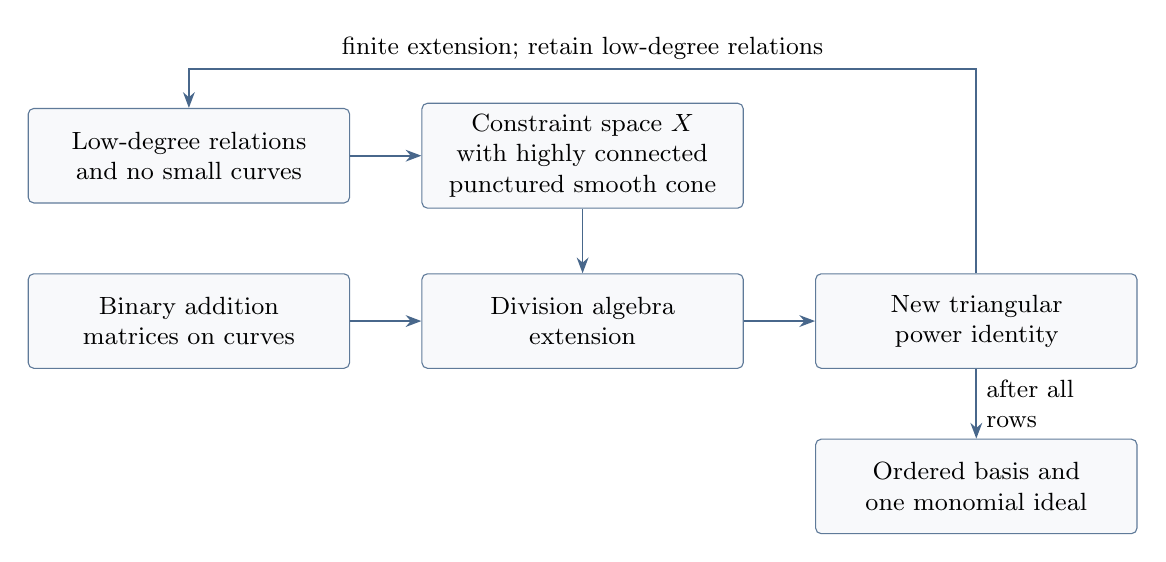
\begin{tikzpicture}[
 box/.style={draw=linkblue!70,rounded corners=2pt,fill=linkblue!3,align=center,text width=38mm,minimum height=12mm,font=\small,inner sep=4pt},
 arrow/.style={-{Stealth[length=2mm]},semithick,draw=linkblue!80},
 every node/.style={font=\small}]
\node[box] (low) at (0,2.1) {Low-degree relations\\and no small curves};
\node[box] (param) at (5,2.1) {Constraint space $X$\\with highly connected\\punctured smooth cone};
\node[box] (curves) at (0,0) {Binary addition\\matrices on curves};
\node[box] (division) at (5,0) {Division algebra\\extension};
\node[box] (row) at (10,0) {New triangular\\power identity};
\node[box] (ideal) at (10,-2.1) {Ordered basis and\\one monomial ideal};
\draw[arrow] (low)--(param);
\draw[arrow] (param)--(division);
\draw[arrow] (curves)--(division);
\draw[arrow] (division)--(row);
\draw[arrow] (row)-- node[right,align=left]{after all\\rows} (ideal);
\draw[arrow] (row.north) -- (10,3.2) -- node[above]{finite extension; retain low-degree relations} (0,3.2) -- (low.north);
\end{tikzpicture}
\caption{The induction separates the geometry of the constraints from the binary addition matrices. The return arrow preserves the hypotheses for the next row; monomial extraction is performed only after the construction is complete.}
\label{fig:construction}
\end{figure}

\FloatBarrier
\subsection{Conventions and standard tools}\label{subsec:conventions}

Every center $k$ used in the construction is a finitely generated field extension of the original $\C$. The degree of a central simple algebra is the square root of its dimension over its center. Linear forms with division-algebra coefficients always commute as whole elements of the polynomial algebra; their individual coefficients need not commute. When new tensor factors are used, we will specify the stronger coefficientwise commutativity available between distinct factors.

Each such $k$ admits an abstract embedding into $\C$: its algebraic closure has the same transcendence degree over $\Q$ as $\C$. These embeddings need not fix the original constants. They are used only for complex topology and numerical base-change comparisons, after the relevant geometric hypotheses have been verified. All actual algebra extensions continue to contain the original $\C$ centrally. In particular, division is proved over the unembedded field by rank divisibility, never inferred from a complex specialization. Embeddings chosen at successive stages need not extend one another.

Projective spaces parameterize lines. For a vector space $U$ of formal forms, $\Sym U$ gives those forms degree one, and its geometric projective zero sets lie in $\PP(U^\vee)$. Polynomial functions $w$ on $U$, in contrast, are evaluated on the forms $\ell\in U$. We distinguish these two roles when using differentiation.

We use standard coherent-sheaf and topological $K$-theory with their usual complex orientations. Pullbacks of coherent classes are derived whenever ordinary pullback is not exact. On smooth quasi-projective varieties, finite locally free resolutions give the corresponding topological $K$-classes. For smooth projective varieties, the Riemann--Roch formulas are
\[
 \chi(V,\alpha)=\int_V\ch(\alpha)\td(V),
 \qquad
 \ch(Rp_*\alpha)=p_*\bigl(\ch(\alpha)\td(T_p)\bigr)
\]
for projection $p$ off a fixed smooth projective factor. These formulas apply to coherent classes, without assuming that their individual higher direct images are locally free; see \cite[Sections~4, 6, and~7]{BorelSerre58}. The singular-space Euler-characteristic argument needed below is proved separately. The integral projective-space basis and complex Thom class in topological $K$-theory are recalled at their point of use from \cite{Hatcher}.

\section{Division coefficients and monomial ideals}\label{sec:reduction}

We first reduce the Hilbert-function problem to identities among commuting
linear forms. Their coefficients will lie in a division algebra, but the
linear forms themselves will commute. This distinction lets us use
commutative algebra to obtain a basis and division-algebra linear algebra
to count its least exponents.

Throughout, a field \(k\) extending the original \(\C\) is identified with
a central subfield of every \(k\)-algebra in use. In
\(\Delta[x_1,\ldots,x_n]\), the variables \(x_j\) are central and have
degree one, and elements of \(\Delta\) have degree zero.

\begin{lemma}[Ordered-basis criterion]\label{lem:ordered-basis}
Let \(f_1,\ldots,f_n\) be a homogeneous regular sequence in
\(S=\C[x_1,\ldots,x_n]\), with \(\deg f_i=a_i>0\).
Suppose that a field extension \(k/\C\) and a finite-dimensional central
division \(k\)-algebra \(\Delta\) have the following property.
There is a finite collection of pairwise commuting elements of
\(\Delta[x_1,\ldots,x_n]_1\), containing \(x_1,\ldots,x_n\), whose
generated commutative \(k\)-algebra \(A\) contains elements
\(t_1,\ldots,t_n\) of degree one satisfying
\begin{equation}\label{eq:triangular}
 t_i^{a_i}
 =c_i f_i+\sum_{l<i}B_{il}f_l+\sum_{d>i}C_{id}t_d,
 \qquad 1\le i\le n,
\end{equation}
where \(c_i\in k^\times\) and all terms are homogeneous, with
\(B_{il},C_{id}\in A\).
Then \(A\) is finite over \(k[x_1,\ldots,x_n]\), and
\[
 \{t_1^{\alpha_1}\cdots t_n^{\alpha_n}:\alpha\in\Z_{\ge0}^n\}
\]
is a basis of \(\Delta[x_1,\ldots,x_n]\) as a left
\(\Delta\)-vector space.
\end{lemma}

\begin{proof}
The regular sequence gives
\begin{equation}\label{eq:regular-hilbert}
 \Hilb_{S/(f_1,\ldots,f_n)}(t)
 =\frac{\prod_{i=1}^n(1-t^{a_i})}{(1-t)^n}
 =\prod_{i=1}^n(1+t+\cdots+t^{a_i-1}).
\end{equation}
Thus the \(f_i\) have no common projective zero, and this remains true
after any field extension.

Put \(N=\Delta[x_1,\ldots,x_n]\), considered as a right \(A\)-module.
The inclusions
\[
 k[x_1,\ldots,x_n]\subseteq A\subseteq N
\]
make \(A\) a submodule of the finite free \(k[x]\)-module \(N\).
Consequently \(A\) is finite over \(k[x]\), and both \(A\) and the finite
right \(A\)-module \(N\) are Noetherian.

We claim that \(t_1,\ldots,t_n\) is an \(N\)-regular sequence.
First, \(A/(t_1,\ldots,t_n)\) is zero dimensional. Indeed, at a geometric
point where all \(t_j\) vanish, the identities
\eqref{eq:triangular}, read in increasing order of \(i\), give
\(f_1=\cdots=f_n=0\). Equation~\eqref{eq:regular-hilbert} then forces
all \(x_j=0\), and finiteness over \(k[x]\) gives the asserted
zero-dimensional quotient.

Let \(\mathfrak m=A_{>0}\), the graded maximal ideal. The central
variables \(x_1,\ldots,x_n\) form an \(N\)-regular sequence because
\(N=\Delta[x]\) is free over \(k[x]\). Localization preserves the
successive injections. Their quotient is \(\Delta\), on which every
positive-degree element of \(A\) acts trivially, so it remains nonzero
on localization. Thus the sequence is also \(N_{\mathfrak m}\)-regular.
The support dimension of \(N_{\mathfrak m}\) is at most \(n\) by
finiteness over \(k[x]\). It therefore equals its depth \(n\).
The system-of-parameters theorem for finite Cohen--Macaulay modules
now implies that \(t_1,\ldots,t_n\) is regular on \(N_{\mathfrak m}\);
see \cite[Proposition~10.103.4, Tag 00N6]{Stacks}.
It is regular on the graded module \(N\) as well. To see the
localization step explicitly, a nonzero homogeneous element of any
graded kernel or quotient cannot be annihilated by an element of
\(A\setminus\mathfrak m\): the nonzero constant term of that element
would survive in the lowest-degree component.

Since all the \(t_j\) have degree one,
\[
 \Hilb_{N/\sum_j Nt_j}(t)
 =(1-t)^n\Hilb_N(t)=\dim_k\Delta.
\]
Its degree-zero part is already \(\Delta\). Hence, in every positive
degree, \(N_d=\sum_jN_{d-1}t_j\). Induction on degree, using
commutativity of the \(t_j\), shows that
\[
 \{\,t^\alpha=t_1^{\alpha_1}\cdots t_n^{\alpha_n}:
          \alpha\in\Z_{\ge0}^n\,\}
\]
spans \(N\) with coefficients on the left in \(\Delta\).
In degree \(d\) its cardinality is
\(\binom{n+d-1}{n-1}=\dim_\Delta N_d\); it is therefore a left
\(\Delta\)-basis.
\end{proof}

The full basis permits a single exponent comparison for every element of
an ideal. We now extract the Hilbert-function consequence; no further
geometric input is needed.

\begin{proposition}[Monomial extraction]\label{prop:monomial-reduction}
Let \(f_1,\ldots,f_n\), \(k\), \(\Delta\), \(A\), and
\(t_1,\ldots,t_n\) satisfy the hypotheses of
Lemma~\ref{lem:ordered-basis}. For every homogeneous ideal
\(I\subseteq S=\C[x_1,\ldots,x_n]\) containing the \(f_i\),
there is one monomial ideal \(J\subseteq S\) such that
\[
 x_i^{a_i}\in J\quad(1\le i\le n),\qquad
 \dim_\C(S/J)_d=\dim_\C(S/I)_d\quad(d\ge0).
\]
\end{proposition}

\begin{proof}
Put \(N=\Delta[x_1,\ldots,x_n]\), with the full left
\(\Delta\)-basis of Lemma~\ref{lem:ordered-basis}.

Extend \(I\) to the two-sided ideal \(\Delta I\) of \(N\). For each
nonzero homogeneous element of this ideal, take the least exponent
in its \(t\)-basis expansion under lexicographic comparison of the
coordinates in the order
\[
 \alpha_n,\alpha_{n-1},\ldots,\alpha_1.
\]
Let \(E\subseteq\Z_{\ge0}^n\) be the set of all such exponents.
Right multiplication by \(t_j\) translates every exponent by the
same vector \(\mathbf e_j\), without moving any left coefficient.
Thus \(E+\mathbf e_j\subseteq E\). In each degree, elimination over
the division algebra \(\Delta\) shows that the number of exponents
in \(E\) is the left dimension of \((\Delta I)_d\).

For each \(i\), Equation~\eqref{eq:triangular} puts
\[
 t_i^{a_i}-\sum_{d>i}C_{id}t_d
\]
in \(\Delta I\). Expand the \(C_{id}\) in the \(t\)-basis with
coefficients on the left. Every exponent in a term \(C_{id}t_d\)
has a positive coordinate of index greater than \(i\), and hence is
strictly larger than \(a_i\mathbf e_i\) in the chosen order.
It follows that \(a_i\mathbf e_i\in E\).

The upward-closed set \(E\) defines a single monomial ideal
\[
 J=\langle\,x^\alpha:\alpha\in E\,\rangle\subseteq S.
\]
It contains the required pure powers. Finally,
\[
 N/\Delta I\simeq \Delta\otimes_\C(S/I)
\]
as graded left \(\Delta\)-vector spaces. The complementary exponent
count in every degree gives the asserted Hilbert function.
\end{proof}

Our task is now to construct \eqref{eq:triangular}, starting with
row \(n\) and proceeding down to row \(1\). At a stage of degree
\(b=a_i\), the constraints on a new sum of \(b\)-th powers involve
the degree-\(b\) part of a formal ideal. We therefore encode earlier,
possibly higher-degree rows as consequences of linear and quadratic
relations, whose generators still have degree at most \(b\).
Section~\ref{sec:low-relations} defines these constraints and proves
the simple-factor property needed for their parameter space.

\section{Low relations and simple factors}\label{sec:low-relations}

At stage \(i\) of the construction, we seek a sum of \(b\)-th powers
that lies in the degree-\(b\) ideal piece allowed by the new triangular
row, where \(b=a_i\). The earlier rows have degrees \(a_d\ge b\);
if we retained them only as equations of those degrees, they need not
contribute to this ideal piece. We instead retain them as consequences
of linear and quadratic relations among an enlarged collection of
formal linear forms.

We first describe the equations on a tuple of summands. Each is obtained
by summing the values of a degree-\(b\) polynomial \(w\) on those
summands. The next section requires every nonzero \(w\) in this linear
system to have an irreducible factor of multiplicity one.
We obtain this condition by excluding curves of bounded degree from
the projective zero set of the relations, and then construct initial
data for which this exclusion holds.

\subsection{The induction data}

Fix the regular sequence from Theorem~\ref{thm:construction}, and put
\[
 D=\bigl(\max_{1\le j\le n}a_j\bigr)^2.
\]
At the beginning of stage \(i\), where \(n\ge i\ge1\), the data are:
\begin{enumerate}[label=\textup{(\roman*)}]
\item a finitely generated field extension \(k/\C\) and a
finite-dimensional central division \(k\)-algebra \(\Delta_0\);
\item a finite-dimensional \(k\)-vector space \(U\), with
\(\dim U\ge3\), containing the formal variables \(x_1,\ldots,x_n\),
and a linear evaluation map
\[
 U\longrightarrow\Delta_0[x_1,\ldots,x_n]_1
\]
whose images commute pairwise and which sends each \(x_j\) to the
corresponding central variable;
\item a homogeneous ideal \(Q\subseteq\Sym_k U\), generated in
degrees one and two, which vanishes under evaluation, such that
\(\Sym_k U/Q\) is finite over \(k[x_1,\ldots,x_n]\);
\item formal elements \(t_d\in U\), for \(d>i\), whose rows
\eqref{eq:triangular} hold in \(\Sym_k U/Q\), with nonzero
coefficients \(c_d\in k\).
\end{enumerate}
In addition, after every algebraically closed field extension, the
closed set
\[
 \mathcal C(Q)=V_+(Q)\subseteq\PP(U^\vee)
\]
contains no integral projective curve of degree at most \(D\).
We call \(\mathcal C(Q)\) the characteristic set of \(Q\).
No smoothness, reducedness, or irreducibility is required of this set.
Polynomial degree in \(\Sym U\) always refers to the formal linear
forms, all of which have degree one.

We use the abstract complex embeddings of Section~\ref{subsec:conventions}
only for topology and numerical comparison; division is always proved
over the current field \(k\).

\subsection{The equations for the next row}

Assume the induction data at stage \(i\), and write \(b=a_i\).
The ideal relevant to the new power identity is
\begin{equation}\label{eq:stage-ideal}
 \mathfrak j=(Q,f_l\ (1\le l\le i),t_d\ (d>i))
       \subseteq\Sym_k U.
\end{equation}
Membership in \(\mathfrak j_b\subseteq\Sym^b U\) means that a
degree-\(b\) form has the shape required on the right side of the new
row, modulo \(Q\), with some scalar coefficient of \(f_i\).
That coefficient need not yet be nonzero. Section~\ref{sec:assembly}
will make it nonzero when choosing the sum of powers.

\begin{lemma}\label{lem:stage-basepoint}
The space \(\mathfrak j_b\) is base-point-free on \(\PP(U^\vee)\).
\end{lemma}

\begin{proof}
Every specified generator of \(\mathfrak j\) has degree at most
\(b\): the generators of \(Q\) have degree at most two,
\(b\ge2\), and \(a_l\le a_i=b\) for \(l\le i\).
At a projective point, a nonzero generator can be multiplied by a
monomial of complementary degree nonzero at that point.
Thus a base point of \(\mathfrak j_b\) would annihilate every
generator of \(\mathfrak j\).

At such a point \(f_l=0\) for \(l\le i\) and \(t_d=0\) for \(d>i\).
The earlier triangular rows, taken in the order
\(i+1,i+2,\ldots,n\), imply successively that the remaining \(f_d\)
also vanish. Equation~\eqref{eq:regular-hilbert} forces all \(x_j\)
to vanish, which is impossible at a point of \(\mathcal C(Q)\)
by finiteness over \(k[x]\).
\end{proof}

For \(\lambda\in(\Sym^b U)^\vee\), define the polynomial on \(U\)
by \(w_\lambda(\ell)=\lambda(\ell^b)\), and put
\begin{equation}\label{eq:stage-annihilator}
 W=\{\,w_\lambda:\lambda|_{\mathfrak j_b}=0\,\}.
\end{equation}
Characteristic zero identifies these functionals with degree-\(b\)
polynomials on \(U\), since pure powers span \(\Sym^b U\).
For any tuple \(\ell_1,\ldots,\ell_M\in U\), we have
\[
 \sum_{m=1}^M\ell_m^b\in\mathfrak j_b
 \quad\Longleftrightarrow\quad
 \sum_{m=1}^M w(\ell_m)=0
 \quad\text{for every }w\in W.
\]
These are the equations on the tuple of summands. To obtain an integral
parameter space with a highly connected smooth cone, Section~\ref{sec:parameters}
will use the condition that each nonzero \(w\in W\) has a factor of
multiplicity one. The next lemma derives that condition from the
absence of small curves in \(\mathcal C(Q)\).

\begin{lemma}\label{lem:simple-factor}
Let \(U\) be a vector space of dimension at least three over a
characteristic-zero field, and let \(b\ge2\).
Suppose that \(Q\subseteq\Sym U\) is generated in degrees one
and two, and that its geometric characteristic set contains no
integral curve of degree at most \(b(b-1)\).
Let \(\mathfrak j_b\subseteq\Sym^b U\) be a base-point-free
subspace containing \((Q)_b\), and define \(W\) by
\eqref{eq:stage-annihilator}.
Then every nonzero element of \(W\), after any algebraically closed
extension, has an irreducible factor of multiplicity one.
\end{lemma}

\begin{proof}
Fix \(w\in W\setminus\{0\}\) over an algebraically closed extension.
We first show that every repeated factor of \(w\) must be linear.
If there were no simple factor, a second gradient-map argument would
then force \(w\) to be a pure power, contradicting base-point-freeness.

For every linear or quadratic generator \(q\) of \(Q\),
the annihilation of
\(q\,\Sym^{b-\deg q}U\) gives the constant-coefficient
differential equation
\begin{equation}\label{eq:annihilator-differential}
 q(\partial)w=0.
\end{equation}
Here a basis of \(U\) identifies its elements with the corresponding
constant differential operators on polynomial functions on \(U\).
This is the differential-operator description of the degreewise
annihilator pairing; see \cite[pp.~1082--1083, Definitions~1--2
and~(5a)]{EmsalemIarrobino95}.

Suppose an irreducible factor \(p\) occurs in \(w=p^r h\) with
\(r\ge2\) and \(p\nmid h\). For a quadratic \(q\), the term of
lowest possible \(p\)-adic order in \(q(\partial)w\) is
\[
 r(r-1)p^{r-2}h\,q(\nabla p)
       \pmod{p^{r-1}}.
\]
For a linear \(q\), it is
\(rp^{r-1}h\,q(\nabla p)\pmod{p^r}\).
Equation~\eqref{eq:annihilator-differential} therefore shows that,
generically on the hypersurface \(p=0\), its projective gradient
belongs to \(\mathcal C(Q)\).

If that gradient map is nonconstant, it has nonzero differential
at some smooth point \(a\) of \(p=0\). Choose a tangent vector \(v\)
at \(a\) detected by this differential, and an ambient tangent vector
\(v_{\perp}\) transverse to the hypersurface. A projective plane through \(a\)
with tangent plane spanned by \(v,v_{\perp}\) cuts the hypersurface in a curve
smooth at \(a\), with tangent line spanned by \(v\). Its component
through \(a\) has degree at most \(\deg p\), and its gradient map is
nonconstant. On the normalization of this component, the partial
derivatives are sections of the pullback of \(\cO(\deg p-1)\).
After removing their common base divisor, they define a morphism
whose pulled-back hyperplane bundle has degree at most
\(\deg p(\deg p-1)\). This degree is the degree of the image curve
times the degree of the morphism onto its image. The integral image
is therefore a curve in \(\mathcal C(Q)\) of degree at most
\(b(b-1)\), a contradiction.
If the gradient map is constant instead, Euler's identity
places the hypersurface \(p=0\) in the hyperplane perpendicular
to that constant gradient. Irreducibility then forces \(p\) to
be linear. Thus every repeated irreducible factor of \(w\) is linear.

Assume, seeking a contradiction, that \(w\) has no simple factor.
We may then write
\[
 w=c\prod_{\nu=1}^r p_\nu^{m_\nu},
 \qquad m_\nu\ge2,
\]
with distinct linear forms \(p_\nu\), and put
\(v_\nu=\nabla p_\nu\in U^\vee\).
The preceding argument gives \([v_\nu]\in\mathcal C(Q)\).
For a quadratic generator \(q\), logarithmic differentiation yields
\[
 \frac{q(\partial)w}{w}
 =
 q\left(\sum_{\nu=1}^r\frac{m_\nu v_\nu}{p_\nu}\right)
 -\sum_{\nu=1}^r\frac{m_\nu q(v_\nu)}{p_\nu^2}.
\]
The left side and each \(q(v_\nu)\) vanish. Together with the
linear differential equations, this proves that the ambient
projective gradient map of \(w\) has image in \(\mathcal C(Q)\).
Here the map is defined on the ambient \(\PP(U)\), not just on
one factor hypersurface. If it is nonconstant, restrict it to a line
along which it varies. The partial derivatives restrict to sections
of \(\cO_{\PP^1}(b-1)\); removing their common zeros gives a
nonconstant morphism whose image has degree at most \(b-1\).
That image is again a forbidden curve in \(\mathcal C(Q)\).

Finally, a constant projective gradient means that all partial
derivatives of \(w\) are proportional to one fixed vector.
After a linear change of coordinates, \(w\) depends on only one
coordinate. Homogeneity gives \(w=c\,p^b\) for a nonzero linear
form \(p\in U^\vee\). The corresponding functional on \(\Sym^b U\)
is, up to the nonzero scalar \(c\), evaluation at \(p\).
Its annihilation of \(\mathfrak j_b\) contradicts base-point freeness.
\end{proof}

The geometric hypothesis has now supplied the required factor property
of \(W\). It remains to produce initial division-algebra data with this
hypothesis and to show that the finite enlargements in the induction
preserve it.

\subsection{Starting with generic square roots}

We construct the initial relations as \(s_\rho^2=q_\rho(x)\), with
independent generic quadrics \(q_\rho\). A curve in their projective
zero set would give a finite cover of a curve in \(\PP^{n-1}\), on
which all the \(q_\rho\) acquire square roots. For a curve of bounded
degree, sufficiently many of these square roots remain independent,
forcing the cover degree to exceed the bound. The following field-of-definition
estimate makes this argument uniform over all such curves.

\begin{lemma}\label{lem:bounded-curve-field}
For integers \(n\ge2\) and \(D\ge1\), there is an integer \(d_*(n,D)\)
with the following property. If \(\Omega\) is an algebraically closed
extension of \(\C\) and
\(Z\subseteq\PP^{n-1}_\Omega\) is an integral curve of degree at most
\(D\), then \(Z\) is defined over an algebraically closed intermediate
field \(F_0\subseteq\Omega\) with
\(\operatorname{trdeg}_\C F_0\le d_*(n,D)\).
\end{lemma}

\begin{proof}
We use the hyperplane-incidence description of the Chow form
\cite[Section~1, Proposition~1.1]{Guerra96}, recalling the argument for
curves to make the field-of-definition bound explicit.
Consider pairs of hyperplanes whose intersection meets \(Z\).
The incidence variety over \(Z\), with the two hyperplanes chosen
through a point of \(Z\), is irreducible of dimension \(2n-3\).
A general pair in its image meets \(Z\) in finitely many points,
so its image is an irreducible divisor in
\((\PP^{n-1})^\vee\times(\PP^{n-1})^\vee\).
Its defining bihomogeneous equation has degree \(\deg Z\) in each
block: for a general first hyperplane, the corresponding divisor
in the second block is the reduced union of the \(\deg Z\)
hyperplanes representing the points of intersection.

This equation recovers \(Z\). A point on \(Z\) has the property that
every pair of hyperplanes through it satisfies the equation.
For a point outside \(Z\), choose a first hyperplane through it
meeting \(Z\) properly, and then a second hyperplane through it
avoiding the resulting finite set. That pair does not satisfy the
equation. This recovery condition is defined over the field of coefficients.
Indeed, on a point chart \(x_a\ne0\), a hyperplane through \(x\) has
coefficient \(h_a=-\sum_{j\ne a}h_jx_j/x_a\). Substitute this expression
and its counterpart for the second hyperplane into the incidence
equation, clear denominators, and set every coefficient in the remaining
hyperplane variables to zero. These finite equations express the recovery
condition on the chart and agree on overlaps. Over the algebraic closure
of the coefficient field, take the reduced structure. In characteristic
zero it is geometrically reduced, so extension to \(\Omega\) gives
exactly \(Z\).

An equation of bidegree \((d,d)\), \(d\le D\), uses at most
\(\binom{n-1+D}{D}^2\) coefficients. Adjoin those coefficients to
\(\C\), then take its algebraic closure inside \(\Omega\).
This proves the claim, for instance with
\(d_*(n,D)=\binom{n-1+D}{D}^2\).
\end{proof}

\begin{proposition}\label{prop:initial-data}
For every \(n\ge1\) and \(D\ge1\), there exist data
\(k,\Delta_0,U,Q\) satisfying conditions \textup{(i)}--\textup{(iii)}
above and the condition on \(\mathcal C(Q)\).
They may be chosen with
\[
 U=\langle x_1,\ldots,x_n,s_1,\ldots,s_m\rangle_k,
 \qquad
 Q=(s_\rho^2-q_\rho(x):1\le\rho\le m),
\]
where \(m\ge2\) and the coefficient vectors of the quadrics \(q_\rho\)
are jointly algebraically independent over \(\C\).
\end{proposition}

\begin{proof}
Choose an even integer \(v_0\) and ordinary linear forms
\(L_1,\ldots,L_{v_0}\in\C[x]_1\) whose squares span \(\C[x]_2\).
Such a choice is possible by polarization, increasing \(v_0\) if
necessary. For an integer \(m\) to be specified, form the skew Laurent
algebra on symbols
\[
 y_{\rho j}^{\pm1},
 \qquad 1\le\rho\le m,\quad 1\le j\le v_0,
\]
in which distinct generators in the same row anticommute and
generators in different rows commute. Ordered Laurent monomials
give a basis: multiplication is defined by reordering and inserting
the prescribed signs. Their leading terms show that this algebra
is a domain.

The squares of the generators are central and algebraically
independent. Localize their Laurent polynomial algebra to
\[
 k=\C(y_{\rho j}^2:1\le\rho\le m,\ 1\le j\le v_0).
\]
The resulting algebra \(\Delta_0\) is a finite-dimensional domain
over \(k\), with basis the monomials whose exponents are zero or one;
it is therefore a division algebra. Its center is exactly \(k\).
Indeed, a parity vector \(\alpha\) in one row commutes with its
\(j\)-th generator precisely when
\(\sum_{l\ne j}\alpha_l=0\) modulo two. Writing
\(T=\sum_l\alpha_l\), these equations give \(\alpha_j=T\) for all
\(j\). Since \(v_0\) is even, they imply \(T=0\) and then
\(\alpha=0\). Applying this in every row proves the claim; linear
independence of the parity monomials prevents cancellations.

Evaluate the new formal forms by
\[
 s_\rho=\sum_{j=1}^{v_0}y_{\rho j}L_j(x).
\]
Forms from different rows commute, and their squares are
\[
 s_\rho^2=q_\rho(x)
 :=\sum_{j=1}^{v_0}y_{\rho j}^2L_j(x)^2.
\]
The full-rank linear map from the independent square variables
to the coefficients of each quadric shows that the coefficient
vectors of the \(q_\rho\) are jointly algebraically independent.
The indicated ideal \(Q\) consists of identities, and its quotient
is finite over \(k[x]\), since every \(s_\rho\) is integral.

This supplies the commuting forms and the quadratic relations.
We now choose \(m\) so that the resulting finite cover contains no
curve of degree at most \(D\).
Over any algebraically closed extension \(\Omega\) of \(k\), the
linear projection
\[
 \mathcal C(Q)_\Omega\longrightarrow\PP^{n-1}_\Omega,
 \qquad [x:s]\longmapsto[x],
\]
is defined everywhere and is finite. Its pullback of \(\cO(1)\)
is the ambient \(\cO(1)\). If \(n=1\), its target is a point,
and there is no curve upstairs. We may then take \(m=2\).

Assume \(n\ge2\), and suppose an integral curve \(T\) of degree at
most \(D\) occurs upstairs. Its image is an integral curve \(Z\);
if the map degree is \(d\), then
\[
 \deg T=d\deg Z.
\]
In particular \(d\le D\) and \(\deg Z\le D\).
Choose a field of definition \(F_0\subseteq\Omega\) for \(Z\)
as in Lemma~\ref{lem:bounded-curve-field}, and write \(d_*=d_*(n,D)\).
Let \(r=\binom{n+1}{2}\), the size of each coefficient block.
Since all \(mr\) coefficients are independent over \(\C\),
their transcendence degree over \(F_0\) is at least \(mr-d_*\).

At least \(m-d_*\) entire coefficient blocks are jointly independent
over \(F_0\). For completeness, scan the blocks, retaining a block
whenever it contributes all \(r\) new independent parameters over
the retained blocks and \(F_0\). Each rejected block contributes at
most \(r-1\) even after all retained blocks have been adjoined.
Indeed, enlarging the field generated by the retained blocks can only
decrease the transcendence degree contributed by a rejected block.
Adjoin all retained blocks first, then the rejected ones.
If \(j\) blocks were rejected, the total transcendence degree would
be at most \(mr-j\), so \(j\le d_*\).

Restrict the retained generic quadrics to \(Z\).
Their zero divisors are nonempty, reduced, supported in the smooth
locus, and pairwise disjoint. They can also be taken disjoint from
the zeros of a fixed coordinate \(x_j\) nonzero on \(Z\).
These are nonempty open conditions on the jointly generic full
quadrics: the complete linear system of quadrics is base-point-free,
separates tangent directions on the smooth curve, and can avoid
each specified finite set. At a zero of the \(\rho\)-th such divisor,
\(q_\rho/x_j^2\) has valuation one, while the other retained
functions have valuation zero. Thus their classes are independent
in \(\Omega(Z)^\times/\Omega(Z)^{\times2}\).
The function field of \(T\) contains square roots of all these
functions, by the equations \(s_\rho^2=q_\rho\).
Consequently
\[
 d=[\Omega(T):\Omega(Z)]\ge2^{m-d_*}
\]
by the elementary degree formula for independent squareclasses.
Choose \(m\ge2\) with \(2^{m-d_*}>D\). This contradicts \(d\le D\)
and proves the proposition.
\end{proof}

\subsection{Preserving the geometric condition}

The initial data now satisfy the required curve exclusion. Each later
stage will enlarge the formal relation algebra by a finite graded
extension, still generated in degree one. The following degree
comparison shows why the same exclusion survives.

\begin{lemma}\label{lem:sparsity-preserved}
Let \(U\subseteq\widetilde U\) be finite-dimensional vector spaces
over a field, and let \(Q\subseteq\Sym U\) and
\(\widetilde Q\subseteq\Sym\widetilde U\) be homogeneous ideals,
with \(Q\subseteq\widetilde Q\).
Suppose that \(\Sym\widetilde U/\widetilde Q\) is finite over
\(\Sym U/Q\). Then the induced projection of characteristic sets
is everywhere defined and finite, and pulls back \(\cO(1)\) to
\(\cO(1)\). In particular, if the first characteristic set contains
no integral curve of degree at most \(D\) after algebraically
closed extension, neither does the second.
\end{lemma}

\begin{proof}
The quotient of the larger graded algebra by all positive-degree
old forms is finite dimensional. Hence no point of its projective
scheme has all old coordinates zero. The finite graded algebra
map therefore induces the stated finite projective morphism,
with the asserted hyperplane bundle. On an integral curve, its
degree equals the degree of its image multiplied by the positive
degree of the restricted morphism. A forbidden curve upstairs
would thus give a forbidden curve downstairs.
\end{proof}

These arguments include \(b=2\), when a repeated factor of a quadratic
would already make it a pure square. They also include \(n=1\):
the auxiliary forms in Proposition~\ref{prop:initial-data} ensure
\(\dim U\ge3\), as required by the factor lemma.

We have constructed the initial induction data and shown that their
curve exclusion survives every finite homogeneous enlargement.
At each stage, \(D\ge b(b-1)\), so Lemmas~\ref{lem:stage-basepoint}
and~\ref{lem:simple-factor} show that every nonzero member of the
space \(W\) in \eqref{eq:stage-annihilator} has a simple factor.
Its equations \(\sum_m w(\ell_m)=0\) are exactly the conditions that
\(\sum_m\ell_m^b\) belong to \(\mathfrak j_b\).
The next section studies their parameter complete intersection.

\section{The parameter complete intersections}
\label{sec:parameters}

The constraints from Lemma~\ref{lem:simple-factor} will be imposed on a
sum of many powers.  Their parameter space must remain integral, and its
smooth cone must have enough connectivity to support a later equivariant
construction.  We prove both properties from the multiplicity-one factor
condition.  All homology and cohomology in this section have integral
coefficients.

The join statement below is the global homogeneous form of the
Thom--Sebastiani phenomenon; compare
\cite[Proposition~4.1 and Appendix]{OhmotoYokura} for a local
nonisolated version. We give the needed global homotopy argument
directly, retaining integral homology throughout.

\begin{lemma}[Nonzero levels and joins]
\label{lem:homogeneous-joins}
Let \(w\) be a nonzero homogeneous polynomial of degree \(b\ge2\) on a
complex vector space \(U\).  Suppose that some irreducible factor of \(w\)
has multiplicity one.  Then \(w^{-1}(1)\) is connected.  For every
\(M\ge1\), the smooth hypersurface
\[
 F_w=\left\{(\ell_1,\ldots,\ell_M)\in U^{\oplus M}:
                 \sum_{m=1}^M w(\ell_m)=1\right\}
\]
has the homotopy type of the join of \(M\) copies of \(w^{-1}(1)\).
Consequently,
\[
 \widetilde H_j(F_w;\Z)=0\qquad(0\le j\le2M-2).
\]
\end{lemma}

\begin{proof}
Projectivization makes \(w^{-1}(1)\) a cyclic cover of degree \(b\) of
\(\PP(U)\setminus\{w=0\}\).  This complement is connected.  A small
meridian around a smooth point of the multiplicity-one factor, away
from all other factors, permutes the \(b\) choices of a root by a
generator of \(\mu_b\).  The monodromy is therefore transitive, proving
connectedness.

For the join assertion, consider nonzero homogeneous polynomials
\(f\) and \(g\), of positive degrees \(a\) and \(c\), in disjoint sets
of variables.  Cover the level \(f(x)+g(y)=1\) by
\[
 V_-=\{\operatorname{Re}f(x)<2/3\},
 \qquad
 V_+=\{\operatorname{Re}f(x)>1/3\}.
\]
On \(V_-\), a continuous \(c\)-th root of \(1-f(x)\) identifies
\(V_-\) with
\[
 f^{-1}\bigl(\{\operatorname{Re}z<2/3\}\bigr)\times g^{-1}(1).
\]
The first factor contracts to the origin by \(x\mapsto tx\),
\(0\le t\le1\), because \(f(tx)=t^a f(x)\).  Similarly,
\(V_+\simeq f^{-1}(1)\).  On the intersection both \(f(x)\) and
\(1-f(x)\) admit continuous roots, giving a homeomorphism
\[
 V_-\cap V_+\simeq
 f^{-1}(1)\times g^{-1}(1)\times
 \{z\in\C:1/3<\operatorname{Re}z<2/3\}.
\]
Under these identifications, the two inclusion maps are homotopic
to the projections onto \(g^{-1}(1)\) and \(f^{-1}(1)\).
The homotopy pushout for this open cover is their join.  Iteration
proves the asserted description of \(F_w\).  The integral homology
formula for joins, including its Tor terms, now gives the stated
vanishing: joining \(M\) connected spaces has no reduced homology
below degree \(2M-1\).  Smoothness of every nonzero homogeneous level
follows from Euler's identity.
\end{proof}

\begin{theorem}[The parameter spaces]
\label{thm:parameters}
Let \(k\) be a field admitting an embedding into \(\C\), let \(U\) be a
finite-dimensional \(k\)-vector space with \(\dim U\ge3\), and let
\[
 W\subseteq\Sym^b(U^\vee),\qquad b\ge2,\qquad s=\dim W.
\]
Assume that every nonzero element of \(W_{\bar k}\) has an irreducible
factor of multiplicity one over an algebraic closure \(\bar k\).
For integers \(h\ge2\) and \(M\ge2h+4s+10\), put \(N_*=M\dim U\)
and define
\[
 \begin{split}
 Y&=\left\{(\ell_1,\ldots,\ell_M)\in U^{\oplus M}:
                 \sum_{m=1}^M w(\ell_m)=0\quad(w\in W)\right\},\\
 X&=\PP(Y)\subseteq\PP(U^{\oplus M}).
 \end{split}
\]
Then \(X\) is a geometrically integral complete intersection of
codimension \(s\), cut out by \(s\) equations of degree \(b\), and
\[
 \operatorname{codim}_X\operatorname{Sing}X
       \ge M-2s+1>h,
\]
with the codimension of the empty locus understood to be infinite.
In particular, a general \(h\)-dimensional projective linear section
is a smooth complete intersection contained in \(X_{\sm}\).

After any embedding \(k\hookrightarrow\C\), let \(Y^o\) be the
nonzero cone over \(X_{\sm}\).  Both \(Y^o\) and its unit-norm
retract are \((M+2h)\)-connected.
\end{theorem}

\begin{proof}
All geometric assertions may be checked after extension to \(\C\).
The multiplicity-one hypothesis persists under this extension.
Indeed forms without a multiplicity-one factor constitute a finite
union of images of projective multiplication maps
\((p_1,\ldots,p_t)\mapsto\prod_\nu p_\nu^{a_\nu}\), with
\(a_\nu\ge2\) and \(\sum_\nu a_\nu\deg p_\nu=b\).
Their intersection with \(\PP(W)\) is empty geometrically over \(k\),
and remains empty after extension.
Write \(r=\dim U\), \(d=N_*-s\), and \(\kappa=M+2h\).
If \(s=0\), then \(X=\PP^{N_*-1}\) and
\(Y^o=\C^{N_*}\setminus\{0\}\simeq S^{2N_*-1}\).
The conclusions follow from \(2N_*-2\ge\kappa\).
Henceforth assume \(s\ge1\).

\emph{Dimension and the singular locus.}
Choose a basis \(w_1,\ldots,w_s\) of \(W\).  A point has defective
Jacobian rank for the defining equations of \(Y\) only if, for some
\([w]\in\PP(W)\),
\[
 \nabla w(\ell_1)=\cdots=\nabla w(\ell_M)=0.
\]
For any nonzero \(w\), its gradient vanishing set has dimension at
most \(r-1\).  The incidence with \(\PP(W)\) therefore bounds the
defective-rank locus in \(U^{\oplus M}\) by
\begin{equation}
 \dim\{\text{defective rank}\}\le N_*-M+s-1.
 \label{eq:parameter-jacobian}
\end{equation}
Every irreducible component of \(Y\) has dimension at least \(N_*-s\).
Since \(M>2s-1\), no component is contained in the locus in
\eqref{eq:parameter-jacobian}.  Full Jacobian rank gives local dimension
\(N_*-s\), so all components have dimension \(d\) and are generically
smooth.  The \(s\) equations thus have height \(s\) in the polynomial
ring and form a regular sequence.  The resulting complete intersection
is Cohen--Macaulay, with no embedded associated primes.  As it is
generically reduced, it is reduced.

Away from the origin, the cone projection is locally a product with
\(\C^\times\), so smoothness of \(Y\) is equivalent to smoothness of
\(X\).  Equation~\eqref{eq:parameter-jacobian} gives
\begin{equation}
 \operatorname{codim}_Y(Y\setminus Y^o)\ge c:=M-2s+1.
 \label{eq:parameter-omitted}
\end{equation}
Here the origin causes no additional restriction: \(d\ge c\).
The same bound applies to \(\operatorname{Sing}X\).
It remains to prove integrality and connectivity; we have not yet
assumed that the smooth locus is connected.

\emph{Homology of the complement.}
A point outside \(Y\) makes some linear combination of the defining
equations nonzero.  Recording that combination replaces the complement
by a space with contractible fibers over it, while exposing the
nonzero hypersurface levels of Lemma~\ref{lem:homogeneous-joins}.
Define the open incidence variety
\[
 \cH=\left\{(\ell,[w])\in\C^{N_*}\times\PP(W):
                         \sum_m w(\ell_m)\ne0\right\}.
\]
Projection to \(\C^{N_*}\setminus Y\) is an affine bundle of rank
\(s-1\).  For a fixed \(\ell\notin Y\), each line \([w]\) in the
fiber has a unique representative satisfying \(\sum_m w(\ell_m)=1\).
Thus the fiber is the affine hyperplane on which the nonzero evaluation
functional on \(W\) equals one.
Consequently this projection is a homotopy equivalence.

Evaluation also defines a map
\[
 p:\cH\longrightarrow
 \mathcal B:=\cO_{\PP(W)}(1)^\times.
\]
The value at \((\ell,[w])\) is the nonzero linear functional on the
tautological line \(kw\) obtained by evaluation at \(\ell\).
Euler's identity shows that \(p\) is a smooth submersion.
Its fibers have complex dimension \(N_*-1\); after choosing a
representative of \([w]\) and rescaling, they are the levels
\(F_w\) of Lemma~\ref{lem:homogeneous-joins}.

The join lemma controls the homology of every fiber of \(p\).
To pass from these individual fibers to \(\cH\), we use direct image
with proper support; we do not require \(p\) to be a locally trivial
fibration.  Fiber homology becomes compact-support cohomology near
the top degree, where the Leray spectral sequence gives the needed
comparison.  Set \(q=2N_*-2\).  Compact-support Poincar\'e duality on
the fibers \cite[Theorem~3.35]{HatcherAT} and
Lemma~\ref{lem:homogeneous-joins} give
\begin{equation}
 R^q p_!\Z=\Z,\qquad
 R^i p_!\Z=0\quad
 \begin{cases}
 i>q,\\
 q-(2M-2)\le i<q.
 \end{cases}
 \label{eq:parameter-support-rows}
\end{equation}
The top sheaf is constant: a submersion
chart over a small base open set supplies an oriented open ball
in each fiber.  Extension by zero maps its top compact-support
orientation class to the positive generator for that fiber.
This gives an isomorphism from the constant sheaf to the top
direct-image sheaf on the open set.  The local isomorphisms agree
by the complex orientation.

The compact-support Leray spectral sequence is
\[
 H_c^a(\mathcal B,R^i p_!\Z)
       \ \Longrightarrow\ H_c^{a+i}(\cH;\Z).
\]
The stalk formula and this spectral sequence follow from proper-support
base change and derived composition
\cite[Theorems~5.9 and~5.10]{SchnurerSoergel16}; maps between the locally
compact Hausdorff spaces here satisfy their hypotheses. Equivalently,
one may compactify \(p\), extend the constant sheaf by zero, and apply
proper base change and Leray. The base is a real \(2s\)-dimensional
manifold, so its compact-support cohomology with coefficients in any
abelian sheaf vanishes above degree \(2s\)
\cite[Proposition~5.1.2(ii)]{Schapira}. In total degree \(q+2s-j\), with
\(0\le j\le2M-2\), only the top row of
\eqref{eq:parameter-support-rows} can contribute.  In fact, the next
possible row is \(i=q-(2M-1)\), which would require
\[
 a\ge2s-j+2M-1>2s.
\]
An outgoing differential from the top row to another nonzero row
has length at least \(2M>2s\), and hence has zero target.  An
incoming differential would come from above the top row.
Poincar\'e duality on \(\cH\) and \(\mathcal B\) therefore yields
\begin{equation}
 H_j(\cH;\Z)\cong H_j(\mathcal B;\Z)
       \qquad(0\le j\le2M-2).
 \label{eq:parameter-complement-homology}
\end{equation}
The punctured line bundle \(\mathcal B\) retracts to
\(S^{2s-1}\).

\emph{Homology of the smooth cone.}
The closed/open compact-support sequence for
\(Y\subseteq\C^{N_*}\), followed by duality on its complement,
gives
\begin{equation}
 H_c^{2d-j}(Y;\Z)
   \cong H_{2s+j-1}(\C^{N_*}\setminus Y;\Z)
   \cong H_{2s+j-1}(\cH;\Z)
 \label{eq:parameter-support-transfer}
\end{equation}
for \(0\le j\le\kappa\).  Both adjacent ambient compact-support
groups vanish, since their degrees are below \(2N_*\).
The homology range in \eqref{eq:parameter-complement-homology}
applies because
\begin{equation}
 2s+\kappa-1\le2M-2.
 \label{eq:parameter-complement-range}
\end{equation}
Removing \(Y\setminus Y^o\) does not change the left side of
\eqref{eq:parameter-support-transfer}. Indeed, a finite filtration of
the removed algebraic set by smooth locally closed strata, together with
the compact-support closed/open sequence, gives vanishing above its real
dimension from the same manifold bound.
Equation~\eqref{eq:parameter-omitted} bounds that dimension by
\(2(d-c)\), whereas
\begin{equation}
 2d-j-1>2(d-c)\quad(0\le j\le\kappa),
 \qquad
 \kappa\le2c-2=2M-4s.
 \label{eq:parameter-removal-range}
\end{equation}
Both \eqref{eq:parameter-complement-range} and
\eqref{eq:parameter-removal-range} follow from
\(M\ge2h+4s+10\).
Duality on \(Y^o\) now gives
\[
 H_0(Y^o;\Z)=\Z,\qquad
 \widetilde H_j(Y^o;\Z)=0\quad(1\le j\le\kappa).
\]
Every irreducible component of \(Y\) meets \(Y^o\) densely.
The smooth loci of distinct components are disjoint, so their
union could be connected only if there is one component.
Thus \(Y\), and hence \(X\), is integral.

\emph{From homology to homotopy.}
The preceding argument leaves only simple connectivity to prove.
The quasi-projective Lefschetz theorem
\cite[Theorem~1.1.3(ii)]{HammLe85} applies to the smooth open
\(X_{\sm}\) in the projective variety \(X\), with deleted algebraic
subset \(\operatorname{Sing}X\).
It states that the smooth open has the homotopy type of a space
obtained from a sufficiently general hyperplane section by
attaching cells of dimension at least the complex dimension
of the open.  Apply the theorem successively, intersecting the deleted
subset with each hyperplane as well.  Each section down to a surface
therefore surjects on the fundamental group of the preceding smooth
open.

Since \(\operatorname{codim}_X\operatorname{Sing}X>h\ge2\),
a general surface linear section avoids the singular locus.
It is a smooth complete intersection \(S_0\subseteq\PP^{s+2}\)
of \(s\) hypersurfaces of degree \(b\).  Such a surface is simply
connected.  To check the usual smooth flag needed here, replace
its defining equations by general invertible linear combinations.
Off their common base locus, Bertini gives smooth successive
intersections.  Along \(S_0\), the independent differentials of
the defining equations give smoothness of every initial
intersection.  Smooth projective Lefschetz, applied to these
very ample divisors, preserves the fundamental group down to
dimension two, starting from projective space.  Therefore
\(\pi_1(S_0)=0\), and the surjections above give
\(\pi_1(X_{\sm})=0\).

The cone \(Y^o\) is the complement of the zero section in
\(\cO_{X_{\sm}}(-1)\).  Its unit circle bundle has a homotopy
exact sequence in which
\(\pi_1(S^1)=\Z\) surjects onto \(\pi_1(Y^o)\), since the base
is simply connected.  Hence \(\pi_1(Y^o)\) is abelian.
Its abelianization is \(H_1(Y^o;\Z)=0\), so it is trivial.
Smooth complex algebraic varieties have CW type.  Successive
applications of the Hurewicz theorem \cite[Theorem~4.32]{HatcherAT}
to the homology vanishing
already proved now give \(\pi_j(Y^o)=0\) for \(1\le j\le\kappa\).

Radial retraction gives the same connectivity for the unit cone.
Finally, the strict bound on the singular codimension and Bertini
give the asserted smooth \(h\)-dimensional sections.
All conclusions hold after every complex embedding and imply the
stated geometric assertions over \(k\).
\end{proof}

We shall use the unit cone
\[
 Y_1=\{y\in Y^o:\|y\|=1\},
\]
with a Hermitian norm that is the orthogonal sum of norms on the
\(M\) blocks.  Common circle scaling and independent multiplication
of the blocks by \(b\)-th roots of unity preserve \(Y\) and its
smooth locus.  The radial retraction \(Y^o\to Y_1\) is equivariant
for these commuting actions.

\section{Curves realizing binary power addition}\label{sec:curves}

We next construct commuting matrix polynomials that replace two inputs by
one output whose \(b\)-th power is their sum.  The matrices vary over a
Picard variety.  An accompanying finite group action, free on a
degree-one Picard variety, will allow the next two sections to control
the division algebra obtained by descent.

All curves in this section are defined over the original field \(\C\).
They may therefore be extended to any of the centers used in the
construction.  For a left group action, transport of line bundles and
sections means \(g_*=(g^{-1})^*\).  In particular the action on
\(\Pic^d(C)\) is \([A]\mapsto[g_*A]\).
A \(G\)-linearization of a line bundle means lifts of the action to its
total space that are linear on fibers and satisfy the group law exactly.
This is stronger than isomorphisms between transported bundles whose
composites agree only up to a scalar.

\begin{proposition}[Binary addition data]\label{prop:binary-curves}
Let \(b\ge2\), fix a primitive \(b\)-th root \(\zeta\), and put
\[
 G=(\mu_b^b/\mu_b)\rtimes(\Z/b),\qquad e=b^b,
\]
where the denominator is the diagonal subgroup and \(\Z/b\) permutes
the \(b\) factors cyclically.  There are smooth connected projective
curves \(C,T_0\), a connected \'etale \(G\)-cover \(C\to T_0\), and a
genuinely \(G\)-linearized line bundle \(L\) on \(C\) with the following
properties.
\begin{enumerate}[label=\textup{(\roman*)}]
\item The genera and degree satisfy
\[
 g_T:=g(T_0)=b-1,\qquad g(C)-1=e(g_T-1),\qquad \deg L=e.
\]
\item There are sections \(a_\alpha\in H^0(C,L)\), indexed by
\(\alpha\in\Z_{\ge0}^b\) with \(|\alpha|=b\), whose transport follows
the degree-\(b\) monomial representation in formal homogeneous
coordinates \(p_0,\ldots,p_{b-1}\). The notation \(p^\alpha\) labels
the section \(a_\alpha\) when \(|\alpha|=b\); it does not assign
individual sections of \(L\) to the \(p_j\). Write \(a_\alpha=p^\alpha\)
and set
\[
 z=\frac1b\sum_{j=0}^{b-1}p_j^b,\qquad
 u=-\frac1b\sum_{j=0}^{b-1}\zeta^{-j}p_j^b,\qquad
 v=p_0\cdots p_{b-1}.
\]
They satisfy
\begin{equation}\label{eq:binary-section-relations}
 p_j^b=z-\zeta^ju,\qquad z^b=u^b+v^b.
\end{equation}
The section \(z\) is invariant, and \(u,v\) have characters
\(\chi,\psi:G\to\mu_b\), respectively.  The pencil \(u,v\) is
base-point-free and defines a degree-\(e\) morphism
\(\pi:C\to\PP^1\) with \(L=\pi^*\cO(1)\).
\item For a generic \(A\in\Pic^0(C)\), over its field of definition
\(\kappa\), the space \(E_A=H^0(C,A L^{g_T})\) has dimension \(e\).
Multiplication of sections gives isomorphisms
\begin{equation}\label{eq:curve-free-module}
 H^0(C,A L^{g_T+j})
   =E_A\otimes_\kappa\Sym^j_\kappa\langle u,v\rangle
       \qquad(j\ge0).
\end{equation}
Every \(a\in H^0(C,L)\) consequently acts by a homogeneous linear
matrix polynomial \(M_a(U,V)\in\End_\kappa(E_A)[U,V]\).
These matrix polynomials commute, preserve all polynomial identities
among the sections, and satisfy
\[
 M_u=U\,\mathrm{id},\qquad M_v=V\,\mathrm{id},\qquad
 M_z^b=(U^b+V^b)\,\mathrm{id}.
\]
Their dependence on \(A\) is algebraic on a nonempty \(G\)-stable
open subset of \(\Pic^0(C)\).  Under transport on this family,
\begin{equation}\label{eq:matrix-transport}
 M_{g_*a}(U,V)
     =(g_{\mathrm{coeff}}M_a)(\chi(g)U,\psi(g)V).
\end{equation}
Here \(g_{\mathrm{coeff}}\) transports the endomorphism coefficients;
scalar choices in identifying transported line bundles have no effect.
\item The action of \(G\) on \(\Pic^1(C)\) is free.  For every character
\(\xi:G\to\mu_b\), there is a continuous map
\(\Pic^1(C)\to S^1\) equivariant for the given \(G\)-action and
multiplication by \(\xi\) on \(S^1\).
\end{enumerate}
\end{proposition}

The three sections \(u,v,z\) give the binary identity. The full monomial
family \(a_\alpha\) also encodes the construction by linear and quadratic
relations in Section~\ref{sec:assembly}, as required by the induction
data of Section~\ref{sec:low-relations}.
We prove the proposition in three steps: a cover with the required
sections, a free module for multiplication by those sections, and the
two properties of the degree-one Picard variety.

\subsection{The cover and its sections}

\begin{lemma}\label{lem:binary-cover}
There are curves, a cover, and a linearized line bundle satisfying
parts \textup{(i)} and \textup{(ii)} of
Proposition~\ref{prop:binary-curves}.
\end{lemma}

\begin{proof}
Inside \(\PP^{b-1}\), with coordinates \(p_0,\ldots,p_{b-1}\), take
the inverse image under coordinate-wise \(b\)-th powering of the line
parameterized by
\[
 [u:z]\longmapsto[z-u:z-\zeta u:\cdots:z-\zeta^{b-1}u].
\]
Thus the preimage is defined by the \(b-2\) independent linear
relations on the \(p_j^b\); no equation is imposed when \(b=2\).
Let \(C'\) be its normalization.  To establish its irreducibility,
put \(s=u/z\).  On the generic fiber over the \(s\)-line the coordinate
ratios satisfy
\[
 (p_j/p_0)^b=\frac{1-\zeta^j s}{1-s},\qquad 1\le j<b.
\]
These \(b-1\) functions generate a free
\((\Z/b)\)-submodule of
\(\C(s)^\times/\C(s)^{\times b}\): valuation at
\(s=\zeta^{-j}\) detects the \(j\)-th exponent independently.
Kummer theory gives a field extension of degree \(b^{b-1}\).
This argument uses valuations equal to one and applies also when
\(b\) is composite.  Every component of the projective preimage
has dimension at least one, since there are \(b-2\) equations, and
the coordinate-power map is finite.  Hence every component dominates
the line.  The integral generic fiber therefore proves that its
reduced support, and consequently \(C'\), is irreducible.

Phase changes of the \(p_j\), together with their cyclic permutation,
act on this curve.  The group before projectivization is
\(\widetilde G=\mu_b^b\rtimes(\Z/b)\).  Its scalar subgroup is the
diagonal \(\mu_b\), and the cyclic permutation already has order
\(b\) before taking the quotient.  Thus the resulting group is
the stated semidirect product \(G\).  Its action is faithful:
a nontrivial cyclic permutation moves \(s\) by a nontrivial
\(b\)-th root, whereas a phase change fixing a general point with
all coordinates nonzero must be diagonal.
The invariant coordinate
\[
 t=s^b
\]
defines a degree-\(b^b\) map \(C'\to\PP^1_t\).  Since \(|G|=b^b\),
this is a Galois cover with group \(G\).

The Kummer cover of the \(s\)-line is ramified precisely at the
\(b\) points \(s=\zeta^{-j}\), with index \(b\).  In particular,
although several of the displayed ratios have a pole at \(s=1\),
their simultaneous adjunction still has local index \(b\): every
unit in \(\C[[x]]\) has a \(b\)-th root, so all local extensions
are contained in \(\C((x^{1/b}))\).
The map is unramified over \(s=0,\infty\).
It follows that the map to the \(t\)-line has exactly the branch
values \(0,1,\infty\), with index \(b\) above each.

Let \(T_0\) be the smooth projective model of
\begin{equation}\label{eq:auxiliary-cyclic-cover}
 d^b=\frac{t(t-1)}{t-2}.
\end{equation}
The valuations of the right side at \(0,1,2,\infty\) are
\(1,1,-1,-1\), respectively.  This is a cyclic degree-\(b\)
cover, totally ramified at those four points and unramified
elsewhere.  Each nontrivial intermediate extension is ramified
at \(2\), whereas \(C'\to\PP^1_t\) is unramified there.
The two Galois extensions are consequently linearly disjoint.
Normalize their fiber product to obtain \(C\).
It is connected, and \(C\to T_0\) remains a \(G\)-cover.

This last cover is \'etale.  Above \(0,1,\infty\), both original
ramification indices are \(b\); in completed local coordinates,
adjoining the same \(b\)-th root of a uniformizer removes the
ramification after normalization.  Above \(2\), and away from
the four listed points, the base change of the original map is
already \'etale.  Riemann--Hurwitz now gives
\[
 2g_T-2=-2b+4(b-1)=2b-4,\qquad
 g(C)-1=|G|(g_T-1).
\]
For \(b=2\), this construction starts with \(C'=\PP^1\) and
produces a degree-four \'etale \(C_2\times C_2\)-cover between
curves of genus one.

Pull \(\cO(b)|_{C'}\) back to \(C\), and call the resulting
bundle \(L\).  The sections \(u,z\) defined in the proposition
have no common zero, since their simultaneous vanishing forces
every \(p_j\) to vanish.  On \(C'\) their pencil is the
degree-\(b^{b-1}\) map to \(\PP^1_s\); hence
\(\deg\cO(b)|_{C'}=b^{b-1}\).  Since \(C\to C'\) has degree
\(b\), we have \(\deg L=b^b=e\).

The standard \(\widetilde G\)-linearization on \(\cO(b)\)
descends to a genuine \(G\)-linearization: a diagonal scalar
in \(\mu_b\) acts trivially in degree \(b\).  Pullback preserves
this linearization.  Degree-\(b\) monomials therefore define
the sections \(a_\alpha\) and their asserted action.
Phase changes fix \(u,z\), cyclic permutation fixes \(z\)
and multiplies \(u\) by a primitive root, and \(v=\prod_jp_j\)
transforms by the product of phases.  This product is invariant
under cyclic permutation and trivial on the diagonal subgroup,
so it defines a character of \(G\).  Denote the resulting
transport characters of \(u,v\) by \(\chi,\psi\).

The equations of the curve give the first relations in
\eqref{eq:binary-section-relations}, and their product gives
\[
 v^b=\prod_{j=0}^{b-1}(z-\zeta^ju)=z^b-u^b.
\]
If \(u=v=0\), this identity gives \(z=0\), which was excluded.
Thus \(u,v\) define a base-point-free pencil.  Its morphism
\(\pi:C\to\PP^1\) satisfies \(L=\pi^*\cO(1)\); since
\(\deg L=e>0\), the morphism is finite of degree \(e\).
\end{proof}

Figure~\ref{fig:curve-covers} summarizes the normalization and its two
projections. It separates the original power-cover geometry from the
base change that removes its ramification.

\begin{figure}[!htbp]
\centering
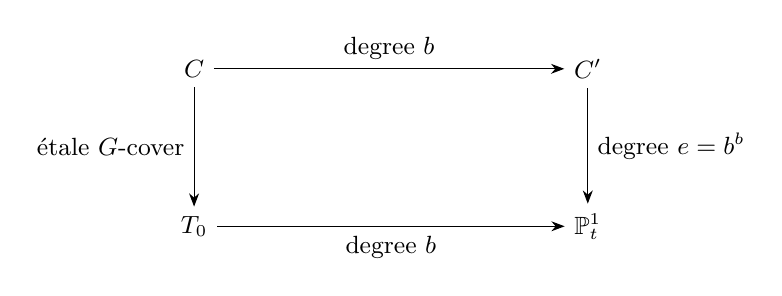
\begin{tikzpicture}[>=Stealth,every node/.style={font=\small}]
\node (C) at (0,2) {$C$};
\node (Cp) at (5,2) {$C'$};
\node (T) at (0,0) {$T_0$};
\node (P) at (5,0) {$\PP^1_t$};
\draw[->] (C)--node[above]{degree $b$}(Cp);
\draw[->] (C)--node[left]{\'etale $G$-cover}(T);
\draw[->] (Cp)--node[right]{degree $e=b^b$}(P);
\draw[->] (T)--node[below]{degree $b$}(P);
\end{tikzpicture}
\caption{The curve $C$ is the normalization of the fiber product.
The lower cover is totally ramified at $0,1,2,\infty$; its ramification
at $0,1,\infty$ cancels that of the right-hand cover, making the
left-hand cover \'etale.}
\label{fig:curve-covers}
\end{figure}
\FloatBarrier

\subsection{Multiplication as linear matrix polynomials}

The cover supplies the required power identity among sections.
We now turn those sections into linear matrix polynomials, with
no choice of basis built into the construction. The use of a trivial
finite pushforward to linearize multiplication is the vector-bundle
description of matrix representations of power identities
\cite{VanDenBergh87,Kulkarni03,CKM12}; we give the needed argument
for this curve and pencil explicitly.

\begin{lemma}\label{lem:binary-matrices}
For the curve and line bundle of Lemma~\ref{lem:binary-cover},
part \textup{(iii)} of Proposition~\ref{prop:binary-curves} holds.
\end{lemma}

\begin{proof}
Let \(g=g(C)\).  For generic \(A\in\Pic^0(C)\), the line bundle
\(A L^{g_T-1}\) is generic of degree
\[
 e(g_T-1)=g-1.
\]
The effective locus in \(\Pic^{g-1}(C)\) is the image of
\(\Sym^{g-1}C\), a projective variety of dimension \(g-1\).
It is a proper closed subset of the \(g\)-dimensional Picard
variety.  Thus \(H^0(C,A L^{g_T-1})=0\), and
Riemann--Roch gives \(H^1(C,A L^{g_T-1})=0\) as well.
Here \(g\ge1\); when \(g=1\), the effective locus in degree
zero consists only of the trivial line bundle.
The complement of this locus, translated to \(\Pic^0(C)\),
is a nonempty \(G\)-stable open subset, because \(L\) is
linearized.

Fix \(A\) in that open set, and put
\[
 \mathcal V=\pi_*(A L^{g_T}).
\]
This is a rank-\(e\) vector bundle on \(\PP^1\): the map
\(\pi\) is finite, and its pushforward is torsion-free on a
smooth curve.  Projection formula and the preceding
vanishing give \(H^*(\PP^1,\mathcal V(-1))=0\).
For every geometric point \(q\in\PP^1\), the exact sequence
\[
 0\longrightarrow\mathcal V(-q)\longrightarrow\mathcal V
   \longrightarrow\mathcal V|_q\longrightarrow0
\]
therefore identifies \(H^0(\PP^1,\mathcal V)\) with
\(\mathcal V|_q\).  It follows that the evaluation map
\[
 H^0(\PP^1,\mathcal V)\otimes\cO_{\PP^1}
       \longrightarrow\mathcal V
\]
is an isomorphism.  This also proves the assertion over the
field of definition of \(A\), since an isomorphism can be
checked after algebraic closure.  In particular
\(\dim E_A=e\).  Tensoring by \(\cO(j)\), taking global
sections, and using projection formula proves
\eqref{eq:curve-free-module}, with its indicated multiplication
map.

Let
\[
 \mathcal M_A=\bigoplus_{j\ge0}H^0(C,A L^{g_T+j}).
\]
Equation~\eqref{eq:curve-free-module} identifies this graded
module canonically with \(E_A\otimes_\kappa\kappa[U,V]\).
Multiplication by a section \(a\) of \(L\) is a homogeneous
degree-one endomorphism of this free module over
\(\kappa[U,V]\).  Such an endomorphism is determined by its
value on degree zero and has the form
\[
 M_a(U,V)=A_aU+B_aV,\qquad A_a,B_a\in\End_\kappa(E_A).
\]
Multiplication of sections is commutative, so these matrix
polynomials commute as elements of \(\End_\kappa(E_A)[U,V]\).
Every polynomial identity among sections acts as the zero
endomorphism and remains an identity among the matrices.
In particular \(u,v\) act as \(U,V\), and the identity for
\(M_z\) follows from \eqref{eq:binary-section-relations}.
This does not assert that all the individual matrices
\(A_a,B_a\) commute.

Choose a point of the constant curve to normalize the
universal line bundle on \(\Pic^0(C)\times C\).
On the open subset just specified, the dimensions of the
section spaces are constant and the higher cohomology
vanishes in every degree \(g_T+j\), \(j\ge0\).
Cohomology and base change, applied to these line bundles along the
proper constant-curve projection, then makes the preceding evaluation
and multiplication maps algebraic in \(A\)
\cite[Lemma~30.22.1, Tag 07VK]{Stacks}. The universal lines are flat
over the Noetherian parameter base, as required there.

Finally, all multiplication maps are natural under transport.
An isomorphism between a transported universal line and
the universal line at the transported parameter is unique
up to a scalar.  It acts by the same scalar on the source
and target section spaces, so the induced transport on
endomorphisms is independent of that choice and composes
as a group action.  Transporting
\[
 m_a:E_A\longrightarrow E_A\otimes\langle u,v\rangle
\]
and using \(g_*u=\chi(g)u\), \(g_*v=\psi(g)v\) gives
\eqref{eq:matrix-transport}.  On the generic parameter
field this is semilinear transport of the coefficients.
\end{proof}

\subsection{The degree-one Picard variety}

The multiplication construction uses \(\Pic^0(C)\).
The next two properties of \(\Pic^1(C)\) provide, respectively,
a free algebraic action for descent and continuous maps
carrying its prescribed characters.

\begin{lemma}\label{lem:picard-free}
If a finite group \(G\) acts freely on a smooth connected
projective complex curve \(C\), then its induced action on
\(\Pic^1(C)\) is free.
\end{lemma}

\begin{proof}
Suppose an element \(g\ne1\), of order \(r\), fixes
\([V]\in\Pic^1(C)\).  Choose an isomorphism \(g_*V\to V\).
Its \(r\)-fold composite is an automorphism of \(V\), hence
a nonzero scalar.  Rescaling the chosen isomorphism by
an \(r\)-th root of the inverse scalar gives a linearization
of \(V\) under \(\langle g\rangle\).
Since this cyclic subgroup acts freely on \(C\), descent
along the degree-\(r\) \'etale cover
\(q:C\to C/\langle g\rangle\) gives \(V=q^*V_0\).
But then \(1=\deg V=r\deg V_0\), a contradiction.
\end{proof}

\begin{lemma}\label{lem:picard-character-maps}
Let \(q:C\to T\) be a connected \'etale \(G\)-cover of smooth
connected projective complex curves.  For every character
\(\xi:G\to\mu_b\), there is a continuous map
\[
 f_\xi:\Pic^1(C)\longrightarrow S^1,\qquad
 f_\xi(g_*A)=\xi(g)f_\xi(A).
\]
\end{lemma}

\begin{proof}
Identify \(\mu_b\) with \(\Z/b\) by exponentiation.
Compose the monodromy of the cover with \(\xi\) to obtain
\(\bar\alpha\in H^1(T;\Z/b)\).
Since \(H_1(T;\Z)\) is free abelian, \(\bar\alpha\) lifts
to a class \(\alpha\in H^1(T;\Z)\).
Represent \(\alpha\) by a harmonic real one-form with
integral periods.  The form
\[
 \omega=\frac1b q^*\alpha
\]
has integral periods on \(C\): the projection of a closed
loop in \(C\) has trivial covering monodromy, so its
\(\alpha\)-period is divisible by \(b\).
It is also harmonic, since \(q\) is holomorphic and
unramified.  Integrating \(\omega\) modulo \(\Z\) and
exponentiating defines a circle-valued map on \(C\).
For a path from \(c\) to \(gc\), the projected loop has
character \(\xi(g)\); choosing the sign of the monodromy
convention accordingly, the map satisfies
\[
 f_C(gc)=\xi(g)f_C(c).
\]
Its differential, expressed as a real one-form after local
lifting to \(\R\), is the \(G\)-invariant form \(\omega\).

The Abel map
\[
 a:C\longrightarrow\Pic^1(C),\qquad c\longmapsto\cO(c),
\]
is equivariant.  By the Jacobian description as the
quotient of the dual space of holomorphic differentials
by the integral period lattice, pullback by \(a\)
identifies translation-invariant real one-forms on
\(\Pic^1(C)\) with harmonic real one-forms on \(C\),
and induces an isomorphism on integral first cohomology;
see \cite[Proposition~2.2 and Theorem~2.5]{MilneJacobian}.
Consequently \(\omega=a^*\widetilde\omega\), where
\(\widetilde\omega\) is translation-invariant with integral
periods.  Integrating \(\widetilde\omega\) gives a continuous
circle-valued map \(f_\xi\) on \(\Pic^1(C)\).  Adjust its
constant so that \(f_\xi\circ a=f_C\).

The action on the Picard torsor is affine.  The difference
between the pullback of \(\widetilde\omega\) under \(g\)
and \(\widetilde\omega\) is translation-invariant and pulls
back by \(a\) to zero, since \(\omega\) is invariant.
Injectivity of this pullback makes the difference zero.
It follows that \(f_\xi(g_*A)/f_\xi(A)\) is constant on the
connected Picard variety.  On the Abel image it equals
\(\xi(g)\), so it has that value everywhere.
\end{proof}

\begin{proof}[Proof of Proposition~\ref{prop:binary-curves}]
Lemma~\ref{lem:binary-cover} supplies parts \textup{(i)}
and \textup{(ii)}, and Lemma~\ref{lem:binary-matrices}
supplies part \textup{(iii)}.
Apply Lemmas~\ref{lem:picard-free}
and~\ref{lem:picard-character-maps} to the \'etale cover
\(C\to T_0\) to obtain part \textup{(iv)}.
\end{proof}

\section{Coherent descent and Euler characteristics}\label{sec:descent}

The matrices in Section~\ref{sec:curves} are defined over a function
field and need not themselves generate a division algebra.  We now
combine them with the parameter complete intersection to obtain a
division algebra that also contains the previous coefficient algebra.
The main step in this section converts the reduced rank of an arbitrary
module into an Euler characteristic.  Section~\ref{sec:index} uses that
conversion to prove the required rank divisibility.

\begin{theorem}\label{thm:division}
Let \(k\) be a finitely generated extension of the original field
\(\C\), and let \(\Delta_0\) be a central division algebra over \(k\)
of degree \(e_0\).  Fix an integer \(b\geq2\), a \(k\)-vector space
\(U\) of dimension at least three, and a subspace
\[
W\subseteq\Sym^b(U^\vee),\qquad s=\dim_k W,
\]
such that every nonzero member of \(W_{\bar k}\) has an irreducible
factor of multiplicity one.  Choose integers \(h,M\) in this order,
with
\begin{equation}\label{eq:division-parameters}
h\geq
\max\bigl(\{2\}\cup
\{\,v_p(e_0)s(p^{v_p(b)}-1):p\mid e_0\,\}\bigr),
\qquad M\geq2h+4s+10.
\end{equation}
Here \(v_p\) is the \(p\)-adic valuation, and the prime-indexed set is
empty if \(e_0=1\).
Define
\[
Y=\left\{(\ell_1,\ldots,\ell_M)\in U^{\oplus M}:
          \sum_{m=1}^M w(\ell_m)=0\quad(w\in W)\right\},
\qquad X=\PP(Y).
\]

Take the curve \(C\), group \(G\), and linearized line bundle \(L\)
of Proposition~\ref{prop:binary-curves} for this \(b\).  Write
\(e=|G|=b^b\) and \(g_T=b-1\), and put
\[
B=\prod_{m=2}^M\Pic^0(C),\qquad
H=G^{M-1},\qquad e_1=|H|.
\]
All products and curves here are over \(k\), and \(H\) acts on the
corresponding Picard factors by transport from the curve.
Choose arbitrary characters
\(\rho_1,\ldots,\rho_M:H\to\mu_b\), and let \(H\) act on the
points of the \(m\)-th block of \(Y\) by \(\rho_m\).
Let \(R\) be an affine space with a faithful linear \(H\)-action.
Set
\[
K=k(B\times X\times R),\qquad F=K^H.
\]
For the generic tuple of degree-zero line bundles \(A_m\), let
\[
E=\bigotimes_{m=2}^M H^0(C_K,A_m\otimes L^{g_T}).
\]
Transport induces a semilinear \(H\)-action on \(\End_K(E)\).
Its fixed algebra
\(\Delta_1=\End_K(E)^H\) is central simple of degree \(e_1\)
over \(F\), and
\begin{equation}\label{eq:division-algebra}
\Delta=(\Delta_0\otimes_k F)\otimes_F\Delta_1
\end{equation}
is a central division algebra of degree \(e_0e_1\).
Its scalar extension to \(K\) identifies with
\(\Delta_0\otimes_k\End_K(E)\); in the corresponding descent action,
\(H\) fixes \(\Delta_0\) pointwise.
\end{theorem}

Theorem~\ref{thm:parameters} applies to the stated \(U,W,h,M\).
In particular, \(X\) is geometrically integral, its singular locus
has codimension greater than \(h\), and its punctured smooth cone
\(Y^o\) is \((M+2h)\)-connected after a complex embedding.
Multiplication of each block by a \(b\)-th root of unity preserves
the defining equations and linearizes \(\cO_X(1)\).
The Picard factors are geometrically integral, so \(K\) is a field.
The action on \(R\) makes the action on \(K\) faithful.  The
fixed-field theorem therefore gives \(\Gal(K/F)=H\).

Choose a point on the constant curve \(C\), and normalize its
universal line bundles along that point.  The generic section
spaces in the theorem have dimension \(e\) by
Proposition~\ref{prop:binary-curves}, so \(\dim_K E=e_1\).
We use left transport \(g_*=(g^{-1})^*\).
Transport of a normalized universal line differs from the universal
line at the transported parameter by a line from the parameter base.
At the generic point an identification is therefore unique up to a
scalar.  Such a scalar disappears on endomorphisms, so transport
gives an actual semilinear action on \(\End_K(E)\).
Galois descent, applied also to multiplication and the unit, gives
the asserted central simple algebra \(\Delta_1\)
\cite[Tag 0CDR]{Stacks}.  This proves all assertions of
Theorem~\ref{thm:division} except that \(\Delta\) is division.
The algebra asserted here is over the generic field \(F\). The section
bundle \(E\) exists on the non-effectivity open in \(B\); no extension
of its endomorphism algebra as an Azumaya algebra over all \(B\times X\)
is needed.

If a central simple algebra has degree \(d\), the dimension of each
finite right module is divisible by \(d\), as one sees after a
splitting extension.  We call the quotient its \emph{reduced rank}.
To prove that the algebra is division, it suffices to show that
every reduced rank is divisible by \(d\): a nonzero proper right ideal
would have reduced rank strictly between \(0\) and \(d\).
Accordingly, fix a finite right \(\Delta\)-module of reduced rank
\(r\).  To prove \(e_0e_1\mid r\), introduce the auxiliary products
over \(k\)
\[
P=\prod_{m=2}^M\Pic^1(C),\qquad Z=B\times P,
\]
with the corresponding transport action of \(H\).
These degree-one Picard factors serve two purposes. Their free action
will make equivariant sheaves descend to a finite quotient, while a
determinant line coupling \(B\) to \(P\) will turn the module's reduced
rank into an Euler characteristic. They are used only in this proof;
the fields \(K,F\) and the algebra \(\Delta\) remain those in
Theorem~\ref{thm:division}. The following proposition records the two
numerical identities that the index argument will compare.

\begin{proposition}\label{prop:rank-to-euler}
For the data of Theorem~\ref{thm:division} and a right
\(\Delta\)-module of reduced rank \(r\), there is a class \(\beta\)
of \(H\)-equivariant coherent sheaves on \(Z\times X\), with a
commuting right \(\Delta_0\)-action, having the following properties.

After any embedding \(k\hookrightarrow\C\), identify
\(\Delta_0\otimes_k\C\) with \(\operatorname{Mat}_{e_0}(\C)\), choose
a primitive matrix idempotent \(\epsilon\), and put
\(\beta'=\beta\epsilon\).
The class \(\beta'\) is still \(H\)-equivariant and is perfect on
\(Z\times X_{\sm}\).  For every \(x\in X_{\sm}(\C)\),
\begin{equation}\label{eq:descent-fiber-index}
\int_Z\ch\bigl(\beta'|_{Z\times x}\bigr)\td(Z)=\pm r.
\end{equation}
The sign depends only on the curve factors, not on the module or on
\(x\).  Before making the complex base change, one has
\begin{equation}\label{eq:descent-twist-divisibility}
p(l):=\frac{\chi(Z\times X,\beta\otimes\cO_X(l))}{e_0}
       \ \in\ e_0e_1\Z\qquad(l\in\Z).
\end{equation}
After complex base change, \(p(l)\) is also the ordinary Euler
characteristic of \(\beta'\otimes\cO_X(l)\).
\end{proposition}

\subsection{Removing the scalar ambiguity in transport}

Pull the given module to \(K\), with its Galois descent action, and
tensor over \(\End_K(E)\) with its standard left module \(E\).
The resulting vector space \(\cF_\eta\), at the generic point of
\[
T=B\times X\times R,
\]
has a commuting right \(\Delta_0\)-action and dimension \(e_0r\).
Tensoring with \(E\) has divided the dimension by \(e_1\).
Its transport has scalar weight one in each of the universal lines
\(A_m\).  We first extend this twisted transport over \(T\).

For \(g\in H\), simultaneous transport on the curve and the parameter
gives two line-bundle families \(g_*A_m,A_m\) representing the same
Picard parameter.  Their Hom bundle is the pullback of a line from
the base. More explicitly, if \(q_m:T\times C\to T\) is projection for
the \(m\)-th curve, put
\[
 J_g=\bigotimes_{m=2}^M(q_m)_*\mathcal{H}om(g_*A_m,A_m).
\]
Each factor is a line bundle, and its pullback is identified with the
corresponding Hom bundle by evaluation. Evaluation and composition give
\begin{equation}\label{eq:hom-line-transport}
J_g\otimes g_*\cF_\eta\simeq\cF_\eta,\qquad
J_g\otimes g_*J_{g'}\simeq J_{gg'}.
\end{equation}
The second isomorphism has its usual associative composition law.
The first is compatible with it: transport of the original module
is genuine, and the only scalar choices occur in the line bundles
used to define \(E\).  The genuine linearization of \(L\) adds no
further ambiguity.

\begin{lemma}\label{lem:twisted-extension}
The generic module \(\cF_\eta\) extends to a coherent
\(\Delta_0\)-module \(\cF\) on \(T\) with compatible isomorphisms
\(J_g\otimes g_*\cF\simeq\cF\).
\end{lemma}
\begin{proof}
Choose finitely many rational sections spanning \(\cF_\eta\), and
let \(\cF_0\) be the coherent subsheaf of rational sections generated
by them and their multiples by a \(k\)-basis of \(\Delta_0\).
For each \(g\), use \eqref{eq:hom-line-transport} to view
\(J_g\otimes g_*\cF_0\) as a coherent subsheaf of rational sections.
Its image is coherent because \(T\) is noetherian.  Let \(\cF\)
be the sum of these finitely many images.  Corrected transport
permutes the summands by the composition law in
\eqref{eq:hom-line-transport}; hence it preserves \(\cF\).
All maps commute with \(\Delta_0\), and their composition identities
hold inside rational sections.  The generic fiber is unchanged.
\end{proof}

Pull \(\cF\) back along the auxiliary factors \(P\), and let \(V_m\)
be their normalized universal degree-one lines. We will cancel the
scalar weight of \(\cF\) with a line bundle on \(Z=B\times P\).
Define
\begin{equation}\label{eq:determinant-correction}
\cD=\bigotimes_{m=2}^M
\left(
 \bigl(\det R\Gamma_C(A_m\otimes V_m)\bigr)^{-1}
 \otimes\det R\Gamma_C(A_m)
 \otimes\det R\Gamma_C(V_m)
\right).
\end{equation}
Here \(R\Gamma_C\) means derived pushforward along the constant
curve, retaining the Picard parameters. The projection is smooth and
proper, and the universal lines are flat over the parameter base;
their derived pushforwards are perfect and commute with base change
\cite[Tag 07VK]{Stacks}.
Their determinant lines use the determinant-of-cohomology formalism of
Knudsen and Mumford \cite{KnudsenMumford76}; the functorial construction
and its compatibility with pullback are recalled in
\cite[Tags 0FJI and 0FJW]{Stacks}.
Each factor in \(\cD\) is the inverse Deligne pairing of \(A_m,V_m\)
tensored with the fixed line \(\det R\Gamma_C(\cO_C)\)
\cite[Construction~7.2, Equation~(7.2.1)]{Deligne87}.
We keep the full determinant expression when defining transport.

\begin{lemma}\label{lem:determinant-descent}
The sheaf \(\cF\otimes\cD\) on \(Z\times X\times R\) has a
genuine \(H\)-equivariant structure commuting with \(\Delta_0\).
Its derived restriction to \(R=0\) defines an equivariant coherent
class \(\beta\) on \(Z\times X\).
Nonequivariantly this class is the tensor product of \(\cD\) with
a class pulled back from \(B\times X\).
\end{lemma}
\begin{proof}
Write \(g_C\) for the genus of \(C\).  For one pair \(A,V\) of
degrees zero and one,
\[
\chi(A)=1-g_C,\qquad
\chi(A\otimes V)=\chi(V)=2-g_C.
\]
A scalar acting on a line inside a determinant of cohomology has
exponent equal to its Euler characteristic.  Thus the corresponding
factor of \(\cD\) has scalar weights
\[
\bigl(-\chi(A\otimes V)+\chi(A),
      -\chi(A\otimes V)+\chi(V)\bigr)=(-1,0)
\]
in \(A,V\).  The first weight cancels the weight one of \(\cF\),
and the second leaves no dependence on identifications of \(V\).
Local choices of line identifications therefore give the same
transport on \(\cF\otimes\cD\). To check the group law, compare the
two successive transports with the composed identifications of the
universal lines. Composition in
\(J_g\otimes g_*J_h\longrightarrow J_{gh}\) is the associative
composition from \(g_*h_*A\) to \(g_*A\) to \(A\).
Functoriality of determinants and the genuine transport of the original
module identify the two maps for these composed choices. Any scalar
change of the \(A\)-identification contributes opposite weights on
\(\cF\) and \(\cD\), and a change of the \(V\)-identification has
weight zero. Thus no scalar cocycle remains, and the maps glue to
genuine equivariance.

The origin of the representation \(R\) is \(H\)-fixed.  Its
immersion in the product has the finite equivariant Koszul
resolution on the linear coordinates of \(R\), even when \(X\)
is singular.  The alternating coherent Tor class of restriction
therefore defines \(\beta\), preserving both actions.  Since
\(\cF\) does not depend on \(P\), the last assertion follows.
\end{proof}

\subsection{Extracting the reduced rank}

Fix a complex embedding.  All varieties in this paragraph are
base changed along it.  The action of \(H\) is now \(\C\)-linear
and fixes the constant algebra \(\Delta_0\otimes_k\C\) pointwise.
Consequently taking the image under right multiplication by
\(\epsilon\) is exact and preserves equivariance.  It divides the
dimension of every finite-dimensional matrix module by \(e_0\).
The product \(B\times X_{\sm}\times R\) is smooth and connected.
On it, \(\cF\) is perfect, and the alternating rank of a locally
free resolution is constantly \(e_0r\).  Derived restriction to
\(R=0\) preserves this rank.  Thus, for each \(x\in X_{\sm}\),
Lemma~\ref{lem:determinant-descent} gives
\begin{equation}\label{eq:beta-fiber-factorization}
\beta'|_{Z\times x}=\operatorname{pr}_B^*\gamma_x\otimes\cD,
\qquad \gamma_x\in K^0(B),\qquad \rk\gamma_x=r.
\end{equation}
This argument uses derived restriction; no flatness of \(\cF\)
over \(R\) is required.

\begin{lemma}\label{lem:mixed-picard-pairing}
For any class \(\gamma\in K^0(B)\),
\[
\int_Z\ch(\operatorname{pr}_B^*\gamma\otimes\cD)\td(Z)
   =\pm\rk\gamma,
\]
where the sign is independent of \(\gamma\).
\end{lemma}
\begin{proof}
It suffices to calculate the determinant correction for one curve.
Write \(a=c_1(A)\), \(v=c_1(V)\), and let \(q\) project off \(C\).
Grothendieck--Riemann--Roch for this smooth proper projection gives
\[
c_1\!\left(\bigl(\det Rq_*(A\otimes V)\bigr)^{-1}
       \otimes\det Rq_*A\otimes\det Rq_*V\right)
       =-q_*(av).
\]
Indeed the signed exponential sum
\(-e^{a+v}+e^a+e^v\) has degree-two part zero and degree-four
part \(-av\); a curve has no degree-four Todd term.

Normalization at the chosen curve point removes pure
parameter-space degree-two components from both universal classes.
The class \(a\) has no pure curve component because \(\deg A=0\).
The pure curve component of \(v\) cannot contribute to \(q_*(av)\).
The resulting class is therefore purely mixed between
\(H^1(\Pic^0(C),\Z)\) and \(H^1(\Pic^1(C),\Z)\).
Tensoring by \(\cO_C(-c_0)\), for the chosen curve point \(c_0\),
identifies the torsor \(\Pic^1(C)\) with \(\Pic^0(C)\); different
choices change this identification by translation, which acts trivially
on integral first cohomology. The universal classes identify these
integral lattices with the curve's first-cohomology lattice: pullback by
an Abel map gives
the mixed component of the diagonal class on \(C\times C\), and
the Abel map induces an integral \(H^1\)-isomorphism.
The intersection form on \(H^1(C,\Z)\) is unimodular.  Hence the
mixed class has a unimodular matrix \(\Lambda\).
This is the cohomological Poincar\'e pairing; the rank extraction below
is the numerical counterpart of the Fourier--Mukai calculation in
\cite[Theorem~2.2 and Example~2.6]{Mukai81}.

More explicitly, if \(d=2g_C\) is the real dimension of either
Picard factor and \(b_i,p_j\) are integral bases, a mixed class
\(\theta=\sum_{i,j}\Lambda_{ij}b_i\wedge p_j\) satisfies
\[
\int_{\Pic^0(C)\times\Pic^1(C)}\frac{\theta^d}{d!}
       =\pm\det\Lambda=\pm1.
\]
The factors for distinct curves form separate blocks, so the same
unit calculation holds on \(Z\).
Each Picard tangent bundle is trivial, giving \(\td(Z)=1\).
To obtain top degree on \(P\) from \(\exp(c_1(\cD))\), one must
already use top degree on \(B\), because every mixed term has
degree one on each side.  Thus every positive-degree term of
\(\ch(\gamma)\) contributes zero.  Only its rank remains.
\end{proof}

Combining \eqref{eq:beta-fiber-factorization} with
Lemma~\ref{lem:mixed-picard-pairing} proves
\eqref{eq:descent-fiber-index}.  It remains to obtain the arithmetic
divisibility of the twists over \(k\), where \(\Delta_0\) is still
division.  We need an Euler-characteristic fact that also applies
to the singular variety \(X\).

\begin{lemma}\label{lem:torsor-euler}
Let \(Q\) be a projective scheme over a field, and let
\(\delta:T'\to Q\) be a torsor under a constant finite group
of order \(a\).  For every coherent-sheaf class \(\alpha\) on \(Q\),
\[
\chi(T',\delta^*\alpha)=a\,\chi(Q,\alpha).
\]
\end{lemma}
\begin{proof}
The vector bundle \(\delta_*\cO_{T'}\) has rank \(a\).
Put \(d=[\delta_*\cO_{T'}]-a\in K^0(Q)\).
Multiplication by \(d\) lowers the dimension-of-support filtration
on the coherent-sheaf group \(G_0(Q)\).
To see this, the successive quotients of that filtration are
generated by integral closed supports
\cite[Lemma~42.23.2, Tag 02S9]{Stacks}; on an integral support the two bundles
in \(d\) have the same rank and are isomorphic on a dense open
set.  Localization therefore puts their difference in smaller
support dimension.  In particular this operator is nilpotent.

The torsor becomes the disjoint union of \(a\) copies of \(T'\)
after pullback to \(T'\), so \(\delta^*d=0\).
The projection formula gives, as operators on \(G_0(Q)\),
\[
(a+d)d=0.
\]
Over \(\Q\), the operator \(a+d\) is invertible by a finite
nilpotent expansion, hence \(d\) acts by zero.
Euler characteristic takes values in \(\Z\), so it kills torsion
and \(\chi(Q,d\alpha)=0\).
Finite pushforward and the projection formula now give the
claimed equality.
\end{proof}

\begin{proof}[Proof of Proposition~\ref{prop:rank-to-euler}]
The construction and the first identity have been established
above.  By Proposition~\ref{prop:binary-curves}, \(H\) acts freely
on \(P\), hence on \(Z\times X\).  Its quotient is a projective
scheme, and the quotient morphism is a finite étale \(H\)-torsor;
existence of the scheme quotient and torsor follows from
\cite[Tag 07S7]{Stacks}, and a product of the translates of an
ample line bundle gives projectivity of the quotient.
Equivariant coherent sheaves descend along this torsor, together
with their commuting \(\Delta_0\)-actions
\cite[Proposition~35.5.2, Tag 023R]{Stacks}. The same holds for
\(\beta\otimes\cO_X(l)\), since \(\cO_X(1)\) is linearized.

Each cohomology group of a descended sheaf is a finite right
module over the division algebra \(\Delta_0/k\), so its
\(k\)-dimension is divisible by \(e_0^2\).
Lemma~\ref{lem:torsor-euler} multiplies its Euler characteristic
by \(|H|=e_1\) on passing upstairs.  Applying this term by term
to the coherent class gives
\[
\chi(Z\times X,\beta\otimes\cO_X(l))\in e_0^2e_1\Z,
\]
which proves \eqref{eq:descent-twist-divisibility}.
Finally, field extension preserves coherent cohomology dimensions
by flat base change \cite[Tag 02KH]{Stacks}, even for a complex
embedding that does not fix the original constants.  Over \(\C\),
idempotent reduction divides these dimensions by \(e_0\), proving
the last assertion.
\end{proof}

We have obtained an Euler characteristic equal to the reduced
rank up to sign, together with divisibility for every algebraic
twist.  The geometry of \(X\) prevents an immediate comparison of
these two statements.  The next section makes that comparison
using the connectivity of \(Y^o\), and completes the proof of
Theorem~\ref{thm:division}.

\section{The equivariant index calculation}\label{sec:index}

We complete the proof of Theorem~\ref{thm:division}.  Retain its notation,
and let \(r\) be the reduced rank of a finite right module over
\[
 \Delta=(\Delta _0\otimes_k F)\otimes_F\Delta _1.
\]
Our objective is to prove \(e_0e_1\mid r\).
Proposition~\ref{prop:rank-to-euler} supplies an \(H\)-equivariant coherent
class \(\beta\) on \(Z\times X\), and its reduction \(\beta'\) after a
complex embedding of \(k\).  It also supplies the two numerical
identities \eqref{eq:descent-fiber-index} and
\eqref{eq:descent-twist-divisibility}.  The first recovers \(r\) from an
Euler characteristic on \(Z\); the second gives divisibility of Euler
characteristics on \(Z\times X\).  We connect them by replacing low
dimensional tests in \(X\) with projective space.

\subsection{Equivariant maps into the smooth parameter space}

Put \(\mathbb T=(S^1)^M\).  The point characters defining the action on
the \(M\) blocks of the cone give a homomorphism
\(\rho:H\longrightarrow\mathbb T\); write \(H'=\rho(H)\).
The group \(\mathbb T\) need not preserve the cone, but its finite
subgroup \(H'\) does.  The \(H'\)-action and scalar multiplication by
\(S^1\) commute on the unit cone
\[
 Y_1=\{y\in Y^o:\|y\|=1\}.
\]
Here the norm is the standard Hermitian norm after the chosen complex
embedding.  Radial retraction from \(Y^o\) onto \(Y_1\) is equivariant
for both actions.  By Theorem~\ref{thm:parameters}, \(Y_1\) is
\((M+2h)\)-connected.

\begin{lemma}\label{lem:index-equivariant-map}
There is an \(H'\)-equivariant map
\[
 \Phi:\mathbb T\times\PP^h(\C)\longrightarrow X_{\sm},
\]
where \(H'\) acts by translation on \(\mathbb T\) and trivially on
\(\PP^h(\C)\).  It has an \(H'\times S^1\)-equivariant lift
\[
 \widetilde\Phi:\mathbb T\times S^{2h+1}\longrightarrow Y_1.
\]
If \(t_0\in\mathbb T\) is fixed and \(\Phi_0(z)=\Phi(t_0,z)\), then \(\Phi\)
is homotopic, as an ordinary map, to \(\Phi_0\) composed with projection
onto \(\PP^h(\C)\), and
\[
 \Phi_0^*\cO_X(-1)\simeq\cO_{\PP^h}(-1).
\]
There is also an \(H\)-equivariant map
\(\vartheta:P\longrightarrow\mathbb T\), for the action through \(\rho\).
\end{lemma}

\begin{proof}
The product of the principal bundles
\(\mathbb T\to\mathbb T/H'\) and
\(S^{2h+1}\to\PP^h(\C)\) is a principal \(H'\times S^1\)-bundle.
An equivariant lift \(\widetilde\Phi\) is a section of its associated
bundle with fiber \(Y_1\).  The base
\((\mathbb T/H')\times\PP^h(\C)\) has a finite CW structure of dimension
\(M+2h\).  Extend a section cell by cell: over an \(a\)-cell the
extension obstruction is a map \(S^{a-1}\to Y_1\), which is
null-homotopic by the connectivity just established.  The initial
choice over zero-cells and extension over one-cells are allowed
because \(Y_1\) is nonempty and path connected.  This constructs
\(\widetilde\Phi\), and passage to the scalar-circle quotient gives \(\Phi\).

To compare \(\Phi\) with \(\Phi_0\), forget \(H'\)-equivariance.
The lifts \(\widetilde\Phi(t,z)\) and \(\widetilde\Phi(t_0,z)\) are sections
of the same circle-associated bundle over
\(\mathbb T\times\PP^h(\C)\).  Construct a homotopy relative to its
two endpoints by extending over cells of the base times \([0,1]\).
This relative CW pair has dimension \(M+2h+1\), so the largest
obstruction belongs to \(\pi_{M+2h}(Y_1)\), which also vanishes.
Projectivizing this homotopy proves the assertion about \(\Phi\).
The circle-equivariant map
\(S^{2h+1}\to Y_1\) obtained at \(t_0\) identifies the associated
tautological line bundles, giving the stated isomorphism for \(\Phi_0\).

Finally, any character of \(H=G^{M-1}\) is a product of characters of
its factors.  Lemma~\ref{lem:picard-character-maps} realizes each
factor character by an equivariant circle-valued map on the
corresponding factor of \(P\).  Multiplying these maps realizes each
coordinate of \(\rho\).  Their product is \(\vartheta\).
\end{proof}

\subsection{An integral family of indices}

To bring \(\beta'\) to projective space, use the maps just constructed.
Writing \(z=(a,p)\in B\times P=Z\), define
\[
 \gamma:Z\times\PP^h(\C)\longrightarrow Z\times X_{\sm},
 \qquad
 \gamma(z,t)=(z,\Phi(\vartheta(p),t)).
\]
This map is \(H\)-equivariant, with trivial action on \(\PP^h\).
Since \(H\) acts freely on \(Z\), the quotient \(V=Z/H\) is smooth
projective, and \(\gamma\) induces a map
\[
 V\times\PP^h(\C)\longrightarrow (Z\times X_{\sm})/H.
\]
The ordinary homotopy from \(\Phi\) to \(\Phi_0\) will later compare
this pullback with an algebraic linear section.  For descent we use
\(\gamma\) itself, because \(\Phi_0\) need not be equivariant.
These maps are continuous, so the pullback class need not be algebraic.
We therefore need integration in topological \(K\)-theory that retains
integer coefficients, beyond the rational Chern-character formula.

We use \(K^0(T)\) for the Grothendieck group of complex topological
vector bundles on a compact space \(T\).  The group extends to the
noncompact smooth varieties below by the same vector-bundle
definition; a coherent class on such a variety defines a class in
this group by a finite locally free resolution.
On \(\PP^h(\C)\), put
\[
 u=1-[\cO_{\PP^h}(-1)]\in K^0(\PP^h(\C)).
\]
The projective bundle formula gives
\begin{equation}\label{eq:index-projective-k}
 K^0(\PP^h(\C))=\Z[u]/(u^{h+1}).
\end{equation}
In particular, the coefficients in this basis are integers, a fact
we need in addition to the rational Chern character.

The integrality statement below is a special case of the differentiable
Riemann--Roch theorem of Atiyah and Hirzebruch
\cite[Theorem~1 and Remark~(2)]{AtiyahHirzebruch59}.
We give the projective-space argument with an explicit choice of Thom
class.

\begin{lemma}\label{lem:index-integral-pushforward}
Let \(V\) be a smooth complex projective variety and let
\(\xi\in K^0(V\times\PP^h(\C))\).  There is a unique
\(I_V(\xi)\in K^0(\PP^h(\C))\) such that
\begin{equation}\label{eq:index-integral-pushforward}
 \ch(I_V(\xi))
   =\int_V\ch(\xi)\td(T_V).
\end{equation}
The integral on the right is integration over the \(V\)-factor.
\end{lemma}

\begin{proof}
Choose a projective embedding \(i:V\hookrightarrow\PP^a(\C)\),
with complex normal bundle \(\nu\).
The complex \(K\)-theory Thom class, followed by extension from a
tubular neighborhood, defines
\[
 i_!:K^0(V\times\PP^h(\C))
        \longrightarrow K^0(\PP^a(\C)\times\PP^h(\C)).
\]
We use the Koszul convention for this Thom class: its restriction
to the zero section of \(\nu\) is
\(\lambda_{-1}(\nu^\vee)\).
If \(x_1,\ldots,x_c\) are the Chern roots of \(\nu\), its Chern
character, divided by the ordinary cohomological Thom class, is
\[
 \prod_{\alpha=1}^c\frac{1-e^{-x_\alpha}}{x_\alpha}
       =\td(\nu)^{-1}.
\]
For completeness, this identity follows on the zero section from
\(\ch(\lambda_{-1}(\nu^\vee))=\prod_\alpha(1-e^{-x_\alpha})\)
and from the Euler class \(\prod_\alpha x_\alpha\).
The splitting principle verifies the identity universally for
sums of line bundles, where the product of the universal Chern
classes is a non-zero-divisor; the Thom isomorphism then gives
the asserted identity before restriction as well.
Consequently
\[
 \ch(i_!\xi)=i_*\bigl(\ch(\xi)\td(\nu)^{-1}\bigr).
\]
The exact tangent-normal sequence now implies
\begin{equation}\label{eq:index-ambient-integration}
 \int_{\PP^a}\ch(i_!\xi)\td(T_{\PP^a})
    =\int_V\ch(\xi)\td(T_V).
\end{equation}

The integral projective bundle formula identifies
\[
 K^0(\PP^a(\C)\times\PP^h(\C))
    =\Z[v,u]/(v^{a+1},u^{h+1}),\qquad
 v=1-[\cO_{\PP^a}(-1)].
\]
Write \(i_!\xi=\sum_{i=0}^a\sum_{j=0}^h c_{ij}v^iu^j\),
with \(c_{ij}\in\Z\).
The number
\[
 \int_{\PP^a}\ch(v^i)\td(T_{\PP^a})
    =\chi\bigl(\PP^a,(1-[\cO(-1)])^i\bigr)
\]
is an integer by Hirzebruch--Riemann--Roch, applied additively to
the finite sum of line-bundle classes \(v^i\).
Thus the left side of \eqref{eq:index-ambient-integration} is the
Chern character of an integral combination of \(1,u,\ldots,u^h\),
which gives \(I_V(\xi)\).
Uniqueness follows because the Chern character is injective on
the torsion-free group in \eqref{eq:index-projective-k}:
if \(H=c_1(\cO(1))\), then \(\ch(u)=1-e^{-H}\) has leading term \(H\),
so these \(h+1\) Chern characters are linearly independent over \(\Q\).
The projective bundle and Thom constructions used here are standard
complex \(K\)-theory, with the Koszul convention for the Thom class
specified above \cite[Proposition~2.24, Theorem~2.25,
and pp.~113--114]{Hatcher}; for the
Riemann--Roch formula see \cite[\S7]{BorelSerre58}.
\end{proof}

For a projective variety and a virtual coherent or algebraic
vector-bundle class, \(\chi\) will always mean the additive Euler
characteristic of that class.  We now apply the preceding lemma
to the equivariant class from Section~\ref{sec:descent}.

\begin{proposition}\label{prop:index-test}
In the setting of Theorem~\ref{thm:division}, let \(r\) be the
reduced rank of any finite right \(\Delta\)-module.
There is a smooth \(h\)-dimensional linear section
\(D_0\subset X_{\sm}\), a complete intersection of \(s\) hypersurfaces
of degree \(b\) in \(\PP^{h+s}(\C)\), and integers
\(q_0,\ldots,q_h\in e_1\Z\) such that \(q_0=\pm r\) and
\begin{equation}\label{eq:index-section-divisibility}
 \sum_{j=0}^h q_j\,
 \chi\!\left(D_0,
       (1-[\cO_{D_0}(-1)])^j\otimes\cO_{D_0}(l)\right)
       \in e_0e_1\Z
       \qquad(l\in\Z).
\end{equation}
\end{proposition}

\begin{proof}
Pull back the topological class of
\(\beta'|_{Z\times X_{\sm}}\) along \(\gamma\) and call the resulting
class \(\sigma\).
This pullback is permitted because the class is perfect on the
smooth open product.

The equivariant coherent class \(\beta'\) descends on the free smooth
quotient \((Z\times X_{\sm})/H\).  That quotient is smooth
quasi-projective, so the descended coherent class has a topological
vector-bundle class.  Pulling it back along the quotient of
\(\gamma\) gives
\(\tau\in K^0(V\times\PP^h(\C))\) whose pullback is \(\sigma\).
Since \(Z\to V\) is an étale covering of degree \(e_1\) and
\(T_Z\) is the pullback of \(T_V\), Lemma~\ref{lem:index-integral-pushforward}
gives
\begin{equation}\label{eq:index-family}
 \int_Z\ch(\sigma)\td(T_Z)
   =e_1\ch(I_V(\tau))
   =\ch\!\left(\sum_{j=0}^h q_j u^j\right),
 \qquad q_j\in e_1\Z.
\end{equation}

Nonequivariantly, Lemma~\ref{lem:index-equivariant-map} makes
\(\gamma\) homotopic to \((z,t)\mapsto(z,\Phi_0(t))\).
The equality \eqref{eq:index-family} therefore computes the same
fiber integral for this latter pullback of \(\beta'\).
Evaluate it at any point of \(\PP^h(\C)\).
Only \(q_0\) remains on the right, whereas
\eqref{eq:descent-fiber-index} gives \(\pm r\) on the left.
Thus \(q_0=\pm r\).

This already gives \(e_1\mid r\).  The stronger divisibility by
\(e_0e_1\) is encoded in the algebraic twist indices \(p(l)\) of
\eqref{eq:descent-twist-divisibility}.  A smooth linear section of \(X\)
retains that divisibility and can also be compared with the
projective-space test.  Put \(d=\dim X\).
Theorem~\ref{thm:parameters} gives
\(\operatorname{codim}_X(X\setminus X_{\sm})>h\).
A general linear section of codimension \(d-h\) therefore misses
the singular locus; Bertini gives a smooth section \(D_0\).
As \(X\) is a complete intersection of \(s\) degree-\(b\) equations,
\(D_0\) has the description in the statement.

Choose \(h+1\) linear forms with no common zero on \(D_0\);
these exist by general position since \(\dim D_0=h\).
They define a morphism
\[
 f:D_0\longrightarrow\PP^h(\C),
 \qquad f^*\cO_{\PP^h}(-1)\simeq\cO_{D_0}(-1).
\]
The inclusion \(j:D_0\hookrightarrow X_{\sm}\) and
\(\Phi_0\circ f\) have circle-equivariant lifts from the unit frame
bundle of this same line bundle to \(Y_1\).
Indeed, choose the indicated line-bundle isomorphisms and normalize
them by their positive fiber norms to identify the unit frame bundles.
The relative section-extension argument in
Lemma~\ref{lem:index-equivariant-map}, now over
\(D_0\times[0,1]\), makes those lifts homotopic:
the real dimension of this base is \(2h+1\), below the available
connectivity bound plus one.
Thus \(j\) and \(\Phi_0\circ f\) are homotopic.

Pulling \eqref{eq:index-family} back by \(f\) now identifies
the fiber integral on \(Z\times D_0\) with
\[
 \ch\!\left(
       \sum_{j=0}^h q_j(1-[\cO_{D_0}(-1)])^j
     \right).
 \tag{\(\ast\)}
\]
Define
\[
 p_{D_0}(l)=
 \chi\!\left(Z\times D_0,
       \beta'|_{Z\times D_0}\otimes\cO_{D_0}(l)\right),
\]
where restriction of a coherent class is derived.
Hirzebruch--Riemann--Roch on the smooth projective product, followed
by \((\ast)\), gives
\begin{equation}\label{eq:index-section-rr}
 p_{D_0}(l)=
 \sum_{j=0}^h q_j\,
 \chi\!\left(D_0,
       (1-[\cO_{D_0}(-1)])^j\otimes\cO_{D_0}(l)\right).
\end{equation}

It remains to retain the original divisibility when passing to
this section.  Recall from \eqref{eq:descent-twist-divisibility}
the integers
\[
 p(l)=\chi(Z\times X,\beta\otimes\cO_X(l))/e_0
       \in e_0e_1\Z.
\]
The \(d-h\) hyperplanes defining \(D_0\) have a Koszul resolution
on \(X\): along \(D_0\) they cut transversely in the smooth locus,
and off their common zero locus the complex is exact because
one of the equations is locally a unit.
Tensoring this resolution derivedly with \(\beta\), and then
passing to the complex embedding and the matrix-idempotent
reduction, yields
\begin{equation}\label{eq:index-koszul-difference}
 p_{D_0}(l)
   =\sum_{a=0}^{d-h}(-1)^a\binom{d-h}{a}p(l-a)
   \in e_0e_1\Z.
\end{equation}
Here cohomology commutes with the field extension, and the
matrix-idempotent reduction divides every cohomology dimension by
\(e_0\).  The particular hyperplanes need only be defined after
that extension: the terms on the right of
\eqref{eq:index-koszul-difference} are the original integer Euler
characteristics.  Combining
\eqref{eq:index-section-rr} and \eqref{eq:index-koszul-difference}
proves \eqref{eq:index-section-divisibility}.
\end{proof}

For the integers in Proposition~\ref{prop:index-test}, put
\[
 Q_*(u)=\sum_{j=0}^h(q_j/e_1)u^j\in\Z[u].
\]
Its constant coefficient is \(Q_*(0)=\pm r/e_1\), and all its twisted
Euler characteristics on \(D_0\) are divisible by \(e_0\).
The remaining step extracts the same divisibility for \(Q_*(0)\).
The dimension \(h\) was chosen precisely to allow the following
finite truncation argument.

\subsection{Truncated polynomial congruences}

\begin{lemma}\label{lem:index-padic-truncation}
Let \(p\) be a prime, let \(v\ge1\), and let
\(A,Q\in\Z[u]\).  Suppose the reduction of \(A\) modulo \(p\)
has exact order \(\nu\ge0\) at \(u=0\).
If \(h\ge v\nu\) and
\[
 A(u)Q(u)=0\pmod{(p^v,u^{h+1})},
\]
then \(p^v\mid Q(0)\).
\end{lemma}

\begin{proof}
We successively construct integer polynomials \(Q_i\),
for \(0\le i\le v\), with \(Q_0=Q\), such that
\[
 Q_i(0)=Q(0)/p^i,\qquad
 A Q_i=0\pmod{(p^{v-i},u^{h-i\nu+1})}
       \quad(0\le i<v).
\]
Suppose \(i<v\) and \(Q_i\) has been constructed.
Modulo \(p\), write \(A=u^\nu B\), where \(B(0)\ne0\).
The power series \(B\) is invertible over \(\Z/p\), so the displayed
congruence forces every coefficient of \(Q_i\) through degree
\[
 m_i=h-(i+1)\nu
\]
to be divisible by \(p\).  This degree is nonnegative because
\(h\ge v\nu\).
Let \(Q_{i+1}\) be the truncation of \(Q_i\) through degree \(m_i\),
divided by \(p\).
It is an integer polynomial and has the required constant
coefficient.  Since
\[
 Q_i-pQ_{i+1}\in u^{m_i+1}\Z[u],
\]
restricting the old congruence to degrees at most \(m_i\) gives
\[
 p A Q_{i+1}=0\pmod{(p^{v-i},u^{m_i+1})}.
\]
Coefficientwise division by \(p\) gives the next congruence
modulo \(p^{v-i-1}\).
At \(i=v-1\), the construction shows directly that
\(Q(0)/p^{v-1}\) is divisible by \(p\).
This proves the conclusion.  The same induction includes
\(\nu=0\), when no degrees are lost.
\end{proof}

\begin{proof}[Completion of the proof of Theorem~\ref{thm:division}]
Use \(D_0\), \(q_0,\ldots,q_h\), and \(Q_*\) just constructed for
the chosen module.
If \(e_0=1\), then \(q_0=\pm r\in e_1\Z\) already gives the required
divisibility, so assume \(e_0>1\).
The Hilbert series of the coordinate ring of the complete
intersection \(D_0\) is
\[
 \frac{(1-t^b)^s}{(1-t)^{h+s+1}}.
\]
Euler characteristics of sufficiently positive twists agree
with Hilbert functions.  Moreover, multiplication by
\((1-[\cO(-1)])^j\) gives the same finite difference as
multiplication of generating functions by \((1-t)^j\), apart
from finitely many initial coefficients.  The coefficients in
these differences are integers.  It follows from
\eqref{eq:index-section-rr} that
\begin{equation}\label{eq:index-hilbert-series}
 \sum_{l\ge0}\frac{p_{D_0}(l)}{e_1}t^l
   =Q_*(1-t)\frac{(1-t^b)^s}{(1-t)^{h+s+1}}+R(t),
 \qquad R(t)\in\Z[t].
\end{equation}
By \eqref{eq:index-koszul-difference}, every coefficient on the
left is divisible by \(e_0\).

Multiply \eqref{eq:index-hilbert-series} by
\((1-t)^{h+s+1}\) and reduce coefficients modulo \(e_0\).
The resulting right side is a polynomial that vanishes
coefficientwise.  We may therefore substitute \(t=1-u\), obtaining
\[
 Q_*(u)\bigl(1-(1-u)^b\bigr)^s
     =0\pmod{(e_0,u^{h+s+1})}.
\]
Define
\[
 A_b(u)=\frac{1-(1-u)^b}{u}\in\Z[u].
\]
Cancelling the common monomial \(u^s\) yields
\begin{equation}\label{eq:index-final-congruence}
 A_b(u)^sQ_*(u)=0\pmod{(e_0,u^{h+1})}.
\end{equation}
This is coefficientwise cancellation of a monomial, valid over
\(\Z/e_0\) even when \(e_0\) is composite.  When \(s=0\), the
factor is \(1\), and the constant coefficient of
\eqref{eq:index-final-congruence} immediately gives
\(e_0\mid Q_*(0)\).

For the general case, fix a prime \(p\mid e_0\) and write
\(v=v_p(e_0)\), \(b=p^a c\), where \(p\nmid c\).
Over \(\Z/p\),
\[
 1-(1-u)^b
   =1-(1-u^{p^a})^c
   =c\,u^{p^a}+\text{terms of higher degree}.
\]
Thus \(A_b(u)^s\) has exact order
\(\nu=s(p^a-1)\) modulo \(p\), with nonzero leading coefficient.
The choice of \(h\) in Theorem~\ref{thm:division} gives
\(h\ge v\nu\).
Apply Lemma~\ref{lem:index-padic-truncation} to
\eqref{eq:index-final-congruence}, reduced modulo \(p^v\), to obtain
\(p^v\mid Q_*(0)\).
This also covers primes not dividing \(b\), for which \(\nu=0\);
no assumption that \(b\) is a prime power has been made.
Doing this for every prime divisor of \(e_0\) gives
\[
 e_0\mid Q_*(0),\qquad
 e_0e_1\mid q_0=\pm r.
\]
The module was arbitrary.  A nonzero proper right ideal of the
central simple algebra \(\Delta\), whose degree is \(e_0e_1\),
would have reduced rank strictly between \(0\) and \(e_0e_1\).
The divisibility just proved excludes such an ideal, so
\(\Delta\) is division.
\end{proof}

\section{Construction of the triangular power identities}
\label{sec:assembly}

We now construct one new triangular identity while preserving the low-degree
relations from Section~\ref{sec:low-relations}.  The division theorem allows
all the binary addition matrices to be used in the same coefficient algebra.
The remaining tasks are to make the final output invariant and to keep the
formal relation algebra finite over the old one.

We first record a binary addition using only linear and quadratic
relations.  The resulting algebra is finite over the input algebra;
Lemma~\ref{lem:sparsity-preserved} will then preserve the condition that
the characteristic set contains no curve of small degree.

\begin{lemma}[Finite extension from the Veronese relations]
\label{lem:veronese-extension}
Let \(b\ge2\), let \(k\) contain a primitive \(b\)-th root of unity
\(\zeta\), and let \(A\) be a commutative \(k\)-algebra with elements \(u,v\).
Introduce symbols \(T_\alpha\), indexed by
\(\alpha\in\Z_{\ge0}^{b}\) with \(|\alpha|=b\), and put
\[
 D_j=T_{b e_j}\quad(0\le j<b),\qquad
 z=\frac1b\sum_{j=0}^{b-1}D_j,\qquad
 u_T=-\frac1b\sum_{j=0}^{b-1}\zeta^{-j}D_j,\qquad
 v_T=T_{(1,\ldots,1)}.
\]
Let \(A'\) be the quotient of \(A[T_\alpha]\) by the relations
\begin{align}
 T_\alpha T_\beta&=T_\gamma T_\delta
       &&\text{whenever }\alpha+\beta=\gamma+\delta,
       \label{eq:veronese-exchanges}\\
 D_j&=z-\zeta^j u_T
       &&(0\le j<b),\qquad u_T=u,\quad v_T=v.
       \label{eq:veronese-linear}
\end{align}
Then \(A'\) is finite over \(A\), and in \(A'\)
\begin{equation}
 z^b=u^b+v^b,\qquad
 T_\alpha^b=\prod_{j=0}^{b-1}D_j^{\alpha_j}.
 \label{eq:veronese-monic}
\end{equation}
If \(A\) is graded and \(u,v\) have degree one, these are homogeneous
relations when each \(T_\alpha\) has degree one; the defining relations
\eqref{eq:veronese-exchanges}--\eqref{eq:veronese-linear} have degrees two
and one.
\end{lemma}

\begin{proof}
The pair exchanges identify any two products of the same number of
symbols whose total exponent vectors agree.  To see this directly,
regard such a product as an allocation of exponent units among factors,
each of total degree \(b\).  Choose the exponent vector desired in the
first factor.  Whenever that factor has an excess in one coordinate and
a deficit in another, some other factor has a unit in the deficient
coordinate.  Exchange this unit for a unit in the excess coordinate.
This is one relation of the form \eqref{eq:veronese-exchanges}.
Once the first factor has its desired vector, leave it fixed and continue
with the remaining factors.

Applying this observation to \(T_\alpha^b\) proves the second identity in
\eqref{eq:veronese-monic}.  In particular,
\[
 v^b=v_T^b=\prod_{j=0}^{b-1}D_j
       =\prod_{j=0}^{b-1}(z-\zeta^j u)=z^b-u^b.
\]
Thus \(z\) is integral over \(A\).  Every \(D_j\) belongs to \(A[z]\), and
the second identity in \eqref{eq:veronese-monic} makes every \(T_\alpha\)
integral over \(A[z]\).  There are finitely many symbols, so \(A'\) is
finite over \(A\).  The grading assertion follows from the displayed
defining relations.
\end{proof}

\begin{proposition}[The induction step]
\label{prop:induction-step}
Fix \(1\le i\le n\).  Suppose that a field \(k\), a central division algebra
\(\Delta_0\) over \(k\), a formal space \(U\), and a low-relation ideal
\(Q\subseteq\Sym_k U\) satisfy the induction conditions of
Section~\ref{sec:low-relations}, with the triangular identities already
constructed for the rows \(d>i\).
Then there are a finitely generated extension \(F/k\), a central division
algebra \(\Delta\) over \(F\), and an enlarged formal space and low-relation
ideal over \(F\) satisfying the same conditions with the rows \(d\ge i\)
constructed.  In particular, the enlarged formal space contains a form
\(t_i\) for which
\begin{equation}
 t_i^{a_i}
 =c_i f_i+\sum_{l<i}B_{il}f_l+\sum_{d>i}C_{id}t_d
 \pmod{Q_{\mathrm{new}}},
 \qquad c_i\in F^\times.
 \label{eq:new-triangular-row}
\end{equation}
All the enlarged formal forms evaluate to mutually commuting linear forms
in \(\Delta[x]\), and the new relation ideal is generated by linear forms
and quadrics.
\end{proposition}

\begin{proof}
Put \(b=a_i\), let \(e_0\) be the degree of \(\Delta_0\), and take
\(\mathfrak j\) and \(W\) as in
\eqref{eq:stage-ideal} and \eqref{eq:stage-annihilator}.
Write \(s=\dim_k W\).
Lemma~\ref{lem:stage-basepoint} gives base-point-freeness of
\(\mathfrak j_b\), and Lemma~\ref{lem:simple-factor} shows that every
nonzero geometric member of \(W\) has a factor of multiplicity one.

\smallskip\noindent
\emph{Parameters and the invariant sum.}
Choose integers in the following order:
\begin{align}
 h&\ge
 \max\left(\{2\}\cup
   \{v_p(e_0)s(p^{v_p(b)}-1):p\mid e_0\}\right),\label{eq:assembly-h}\\
 M&\ge
 \max\left\{2h+4s+10,\ \dim_k\Sym^b_k U\right\}.
 \label{eq:assembly-M}
\end{align}
The prime-indexed set in \eqref{eq:assembly-h} is empty if \(e_0=1\).
Theorem~\ref{thm:parameters} supplies the geometrically integral
projective constraint variety
\[
 X=\PP\left\{(\ell_1,\ldots,\ell_M)\in U^{\oplus M}:
           \sum_{m=1}^M w(\ell_m)=0\ \text{for every }w\in W\right\}.
\]
Use the curve and its two characters \(\chi,\psi\) from
Proposition~\ref{prop:binary-curves}.  For \(M-1\) copies of the curve,
indexed by \(m=2,\ldots,M\), let
\[
 H=G^{M-1},\qquad e_1=|H|,
\]
and write \(\chi_m,\psi_m:H\to\mu_b\) for the corresponding characters.
Define characters recursively by
\begin{equation}
 \lambda_M=1,\qquad
 \lambda_{m-1}=\lambda_m\chi_m\quad(M\ge m\ge2),\qquad
 \eta_1=\lambda_1,\quad \eta_m=\lambda_m\psi_m\quad(m\ge2).
 \label{eq:assembly-weights}
\end{equation}
Let \(H\) act on block \(m\) of the constraint cone by the point character
\(\eta_m^{-1}\).
This preserves its equations because their degree is \(b\), and it gives
the natural linearization of \(\cO_X(1)\).

As in Theorem~\ref{thm:division}, put
\[
 B=\prod_{m=2}^M\Pic^0(C),\qquad
 K=k(B\times X\times R),\qquad F=K^H,
\]
where \(R\) is an affine space with a faithful linear \(H\)-action.
Then \(K/F\) is Galois with group \(H\).
Let \(E=\bigotimes_{m=2}^M E_{A_m}\), of dimension \(e_1\) over \(K\),
and let \(\Delta_1\) be the descent of \(\End_K(E)\).
Theorem~\ref{thm:division}, applied with the block characters just chosen,
makes
\begin{equation}
 \Delta=(\Delta_0\otimes_k F)\otimes_F\Delta_1
 \label{eq:assembly-division}
\end{equation}
a division algebra.  Its scalar extension to \(K\) is
\(\Delta_0\otimes_k\End_K(E)\), and \(H\) fixes \(\Delta_0\) pointwise.
Notice that \(e_0,s,b\) were fixed before \(h\), and \(M\) before \(e_1\);
there is no restriction involving the new degree \(e_1\) in
\eqref{eq:assembly-h}.

The generic fiber of \(\cO_X(1)\), pulled back to \(K\), is a
one-dimensional semilinear \(H\)-space.  By Galois descent it has a nonzero
invariant generator \(\tau\).
Choose a \(k\)-basis of \(U\).  In each cone block, divide its coordinate
sections by \(\tau\) and use the resulting coefficients to form
\(\ell_m\in U_K\).
Transport of a coordinate section is pullback by \(g^{-1}\).
The inverse point action \(\eta_m^{-1}\) therefore gives
\begin{equation}
 g\ell_m=\eta_m(g)\ell_m.
 \label{eq:leaf-weights}
\end{equation}
In particular, dividing by the invariant \(\tau\) does not reverse the
character.

The constraint equations say that
\[
 S_b:=\sum_{m=1}^M\ell_m^b\in(\mathfrak j_K)_b.
\]
Since every \(\eta_m^b=1\), the element \(S_b\) is invariant and belongs to
\((\mathfrak j_F)_b\).
We claim that it has a decomposition
\begin{equation}
 S_b=c_i f_i+\sum_{l<i}B_{il}f_l+\sum_{d>i}C_{id}t_d
          \pmod{Q_F},\qquad c_i\in F^\times.
 \label{eq:invariant-sum}
\end{equation}
For this, let
\[
 V_b=Q_b+
       \sum_{l<i}f_l\Sym^{b-a_l}_k U+
       \sum_{d>i}t_d\Sym^{b-1}_k U.
\]
Then \(\mathfrak j_b=V_b+kf_i\).
If \(f_i\in V_b\), any prescribed nonzero coefficient of \(f_i\) may be
absorbed by changing the term in \(V_b\), proving the claim.

Suppose instead that \(f_i\notin V_b\).
Pure \(b\)-th powers span \(\Sym^b U\) in characteristic zero.
Over an algebraic closure, express \(f_i\) as a linear combination of at
most \(\dim\Sym^b U\) such powers, absorb each scalar into a \(b\)-th root,
and pad with zero forms.  The bound \eqref{eq:assembly-M} gives a nonzero
cone point with
\(\sum_m\ell_m^b=f_i\).
Thus the homogeneous coefficient of the class of \(f_i\) in
\(\mathfrak j_b/V_b\) is not identically zero on \(X\).
Geometric integrality makes it nonzero at the generic point.
Dividing all the coordinates by \(\tau\) only multiplies that coefficient
by a nonzero scalar to the \(b\)-th power.
Finally, the spaces \(V_b\) and \(\mathfrak j_b\) are defined over \(k\).
Invariant linear algebra over \(F\) gives
\eqref{eq:invariant-sum}, with homogeneous multipliers of the indicated
degrees.

\smallskip\noindent
\emph{The chain of binary additions over \(K\).}
We next enlarge the formal space over \(K\), keeping the old equations.
Start with \(s'_1=\ell_1\).
In link \(m\), introduce a fresh symbol \(T_{m,\alpha}\) for every
degree-\(b\) monomial \(p^\alpha\) in the curve coordinates.
Each symbol has formal degree one.
Evaluate it by the multiplication matrix from
Proposition~\ref{prop:binary-curves}, on the \(m\)-th tensor factor of \(E\),
with substitution
\begin{equation}
 U_1=s'_{m-1},\qquad U_2=\ell_m.
 \label{eq:link-substitution}
\end{equation}
Let \(s'_m\) be the formal linear combination of the diagonal symbols
corresponding to \(z\).

These substitutions preserve commutativity of the entire list.
Indeed, the coefficient matrices of a new link commute coefficientwise
with \(\Delta_0\) and with the earlier tensor factors.
The two inputs in \eqref{eq:link-substitution} commute with one another
and with all earlier forms.
The inputs therefore centralize the new coefficient algebra
\(\End_K(E_{A_m})\), embedded in the \(m\)-th tensor factor.
Consequently substitution defines a \(K\)-algebra homomorphism
\[
 \begin{aligned}
 \End_K(E_{A_m})[U_1,U_2]
 &\longrightarrow
 \bigl(\Delta_0\otimes_k\End_K(E)\bigr)[x_1,\ldots,x_n],\\
 U_1&\longmapsto s'_{m-1},\qquad U_2\longmapsto\ell_m,
 \end{aligned}
\]
where the inputs on the right denote their evaluated forms.
It preserves the polynomial commutation identities of the new
multiplication matrices, and every new evaluated form commutes with
every earlier one.
This argument uses no coefficientwise commutativity among the matrices
within a single link.

For each link impose the pair-exchange quadrics
\eqref{eq:veronese-exchanges}, the diagonal relations
\eqref{eq:veronese-linear}, and the identifications
\[
 u_T=s'_{m-1},\qquad v_T=\ell_m.
\]
They are identities under evaluation because they are identities of
sections on the curve.
Lemma~\ref{lem:veronese-extension} shows that the resulting quotient is
finite over the preceding formal relation algebra and gives
\[
 (s'_m)^b=(s'_{m-1})^b+\ell_m^b.
\]
After all links, the formal quotient is finite over
\(\Sym_K U_K/Q_K\), is defined by the old and new linear and quadratic
relations, and satisfies
\begin{equation}
 (s'_M)^b=\sum_{m=1}^M\ell_m^b=S_b.
 \label{eq:telescoping-links}
\end{equation}

\smallskip\noindent
\emph{Equivariance and descent.}
Give the new symbol space in link \(m\) the degree-\(b\) action on the
\(p\)-monomials from Proposition~\ref{prop:binary-curves}, multiplied by
the character \(\lambda_m\), and extend it semilinearly over \(K\).
Keep \(U\) fixed.
The pair-exchange relations are stable under the monomial phase and
permutation action and under the common twist.
The diagonal relations are stable as well.
The distinguished symbols \(u_T,v_T,z\) have respective weights
\[
 \lambda_m\chi_m=\lambda_{m-1},\qquad
 \lambda_m\psi_m=\eta_m,\qquad
 \lambda_m.
\]
These are the weights of their prescribed inputs and output:
the input identifications are stable by induction, starting from
\eqref{eq:leaf-weights}.  Thus the full ideal of linear and quadratic
relations is stable.

Evaluation is equivariant, not merely the relation ideal.
For a section \(a\) before the twist, write
\(M_a(U_1,U_2)\) for its linear multiplication matrix.
The transport identity \eqref{eq:matrix-transport} reads
\[
 M_{g_*a}(U_1,U_2)
 =(g_{\mathrm{coeff}}M_a)
      \bigl(\chi_m(g)U_1,\psi_m(g)U_2\bigr),
\]
where \(g_{\mathrm{coeff}}\) includes the field action and transport on
the corresponding endomorphism factor.
Scalar choices in transporting the universal line cancel on these
endomorphisms.
Using the weights of the two inputs and the degree-one homogeneity of
the matrix polynomial, we obtain
\begin{align*}
 g\!\left(M_a(s'_{m-1},\ell_m)\right)
 &=(g_{\mathrm{coeff}}M_a)
       \bigl(\lambda_m(g)\chi_m(g)s'_{m-1},
             \lambda_m(g)\psi_m(g)\ell_m\bigr)\\
 &=\lambda_m(g)\,M_{g_*a}(s'_{m-1},\ell_m).
\end{align*}
This is exactly the action assigned to the twisted symbol.
It proves equivariance successively through all the links.

Take invariant vector spaces under semilinear Galois descent.
The enlarged formal space descends to an \(F\)-space containing \(U_F\),
and the full degree-one and degree-two pieces of the stable relation
ideal descend to finite-dimensional spaces over \(F\). Let
\(Q_{\mathrm{new}}\) be the ideal generated by these descended spaces.
Scalar extension commutes with the multiplication maps generating this
ideal. Since the original relation ideal was generated in degrees one
and two, extension to \(K\) recovers exactly that ideal.
Equivariant evaluation takes these invariant forms into
\(\Delta[x]\), with \(\Delta\) as in \eqref{eq:assembly-division}.
They are mutually commuting.

The last output \(s'_M\) is invariant because \(\lambda_M=1\); define
\(t_i=s'_M\).
Combining \eqref{eq:invariant-sum} with
\eqref{eq:telescoping-links} proves \eqref{eq:new-triangular-row}.
All earlier equations are retained, so every old triangular identity
continues to hold modulo \(Q_{\mathrm{new}}\).

It remains to check the other induction conditions.
Finiteness of the new relation algebra over the old one can be checked
after the faithfully flat extension \(F\subset K\), where it was proved
link by link.  In particular it remains finite over \(F[x]\).
Lemma~\ref{lem:sparsity-preserved} now preserves the geometric
no-small-curve condition: the linear projection of the new
characteristic set is finite and pulls back the old hyperplane bundle.
The central variables still evaluate to themselves, and the formal space
still contains \(U_F\).
Finally \(K\) is finitely generated over \(k\), and so is its finite-group
invariant field \(F\).
Thus the center is still finitely generated over the original
\(\C\), and all induction conditions have been verified.
\end{proof}

\begin{proof}[Proof of Theorem~\ref{thm:construction}]
Proposition~\ref{prop:initial-data} supplies the initial data with no
triangular rows yet constructed.
Apply Proposition~\ref{prop:induction-step} in the order
\(i=n,n-1,\ldots,1\).
Every step retains all preceding identities as consequences of an ideal
generated in degrees at most two.  Thus a later, smaller value of \(a_i\)
does not lose an earlier power identity.
After finitely many steps we have the division algebra and commuting
linear forms satisfying \eqref{eq:triangular} for all \(i\).
Let \(A\) be the commutative graded algebra generated by all the evaluated
formal forms. The center is
finitely generated over \(\C\), all multipliers in the triangular
identities belong to \(A\) in the stated degrees, and all \(c_i\) are
nonzero. Lemma~\ref{lem:ordered-basis} gives finiteness over \(k[x]\)
and the full ordered left-\(\Delta\) basis. This proves every assertion
of Theorem~\ref{thm:construction}.
\end{proof}

\begin{proof}[Proof of Corollary~\ref{thm:main}]
Apply Theorem~\ref{thm:construction} to the regular sequence contained
in \(I\). Proposition~\ref{prop:monomial-reduction} gives one monomial
ideal \(J\) containing all \(x_i^{a_i}\) and having the same Hilbert
function as \(I\) in every degree.
\end{proof}

\section{Generality and consequences}\label{sec:consequences}

The construction and monomial extraction prove Artinian EGH over
\(\C\). We first extend that Hilbert-function conclusion to the scope
of Corollary~\ref{cor:characteristic-zero}, and then derive two further
consequences. These arguments use the EGH conclusion rather than any
additional division-algebra construction.

\subsection{Regular sequences over characteristic-zero fields}
\label{subsec:generality}

\begin{proof}[Proof of Corollary~\ref{cor:characteristic-zero}]
If \(I=S_F\), take \(J=S_F\). Otherwise, first work over \(\C\).
Choose a linear coordinate change for which
\(f_1,\ldots,f_c,x_{c+1},\ldots,x_n\) is regular. The images
\(\overline f_1,\ldots,\overline f_c\) in
\(\C[x_1,\ldots,x_c]\) form a full regular sequence.
Corollary~\ref{thm:main} applies to these images and, more generally,
to every full regular sequence of the prescribed degrees in \(c\)
variables and every homogeneous ideal containing it. This universal
assertion is the premise of the Artinian reduction of
Caviglia--Maclagan \cite[Proposition~10]{CM08}, which gives the desired
Hilbert-function comparison for every ideal containing the original
sequence in \(n\) variables. The lexicographic embedding modulo \(P_F\) gives the stated
lex-plus-powers choice; this reduction and its lex formulation are also
recalled in \cite[Section~4]{CK14}.

For general \(F\), choose homogeneous generators of \(I\) and let
\(F_0\subseteq F\) be the subfield generated over \(\Q\) by their
coefficients and those of the \(f_i\). Let \(I_0\subseteq F_0[x]\) be
generated by those generators together with the \(f_i\). Then
\(I_0F[x]=I\), and faithful flatness of \(F/F_0\) descends regularity
of the sequence to \(F_0[x]\). Embed the finitely generated field
\(F_0\) into \(\C\) and apply the complex case after scalar extension.
Define a monomial ideal over \(F_0\), and then over \(F\), using the same
monomial exponents as the resulting complex ideal. Dimensions of graded
pieces commute with both field extensions from \(F_0\), so the Hilbert
equalities descend to \(F\). The same observation identifies the
degreewise lex-plus-powers choice.
\end{proof}

The companion paper proves the stronger graded Betti inequalities in
this same characteristic-zero scope
\cite[Corollary~1.2]{BettiCompanion}, using the Artinian LPP reduction
of Caviglia--Kummini \cite[Theorem~4.1]{CK14}. The construction in
Theorem~\ref{thm:construction} itself remains the stated construction
for a full complex regular sequence.

\subsection{Local cohomology}

Caviglia--Sbarra's conditional theorem
\cite[Theorem~4.4]{CavigliaSbarra13} also gives a local-cohomology
comparison for the same lex-plus-powers ideal.

\begin{corollary}[Lex-plus-powers extremality for local cohomology]
\label{cor:local-cohomology}
Let \(F\) be a field of characteristic zero, let
\(S_F=F[x_1,\ldots,x_n]\) be standard graded, and put
\(\mathfrak m=(x_1,\ldots,x_n)\). Let
\[
 1\le c\le n,\qquad 2\le a_1\le\cdots\le a_c,
 \qquad P_F=(x_1^{a_1},\ldots,x_c^{a_c}).
\]
Suppose that a homogeneous ideal \(I\subseteq S_F\) contains a homogeneous
regular sequence \(f_1,\ldots,f_c\) with \(\deg f_k=a_k\). Let \(J\) be the
lex-plus-powers ideal prescribed by Corollary~\ref{cor:characteristic-zero}
for \(P_F\), the order \(x_1>\cdots>x_n\), and the Hilbert function of
\(S_F/I\). For this single ideal,
\[
 \dim_F H^i_{\mathfrak m}(S_F/I)_j
 \le
 \dim_F H^i_{\mathfrak m}(S_F/J)_j
 \qquad(i\ge0,\ j\in\Z).
\]
\end{corollary}

\begin{proof}
If \(I=S_F\), both sides vanish. Otherwise, since \(F\) is infinite,
complete \(f_1,\ldots,f_c\) to a regular sequence by \(n-c\) linear forms.
After a linear change of coordinates, the images
\(\overline f_1,\ldots,\overline f_c\) in
\(\overline S=F[x_1,\ldots,x_c]\) form a full regular sequence of the same
degrees. The list of added linear forms is empty when \(c=n\).

Corollary~\ref{cor:characteristic-zero}, applied in \(\overline S\) to every
homogeneous ideal containing this sequence, supplies precisely the Artinian
EGH premise of Caviglia--Sbarra \cite[Theorem~4.4]{CavigliaSbarra13}.
Their Clements--Lindstr\"om image of \(I/(f_1,\ldots,f_c)\) in \(S_F/P_F\)
has preimage \(J\) in \(S_F\). The base-independence identification used
there gives local cohomology with support in \(\mathfrak m\), and their
Hilbert-series comparison is coefficientwise in the full internal
\(\Z\)-grading for every cohomological degree \(i\ge0\). This gives the
displayed inequalities directly over \(F\).
\end{proof}

When \(c<n\), this statement includes positive-dimensional quotients.
When \(c=n\), both quotients are Artinian: their zeroth local cohomology
is the quotient itself and their higher local cohomology vanishes, so the
comparison reduces to the Hilbert-function equality.

\subsection{Quadratic Cayley--Bacharach}

The quadratic case also gives the following scheme-theoretic
Cayley--Bacharach consequence.

\begin{corollary}[Quadratic Cayley--Bacharach]
\label{cor:quadratic-cayley-bacharach}
Let \(F\) have characteristic zero, let \(r\ge1\), and let
\(\Omega\subseteq\PP^r_F\) be a zero-dimensional scheme-theoretic complete
intersection of \(r\) quadrics, of degree \(2^r\). For an integer
\(1\le k\le r\) and a degree-\(k\) hypersurface \(X\subseteq\PP^r_F\),
\[
 \Omega\not\subseteq X
 \quad\Longrightarrow\quad
 \deg(\Omega\cap X)\le 2^r-2^{r-k}.
\]
Equivalently, if \(X\) contains a closed subscheme of \(\Omega\) of degree
strictly greater than \(2^r-2^{r-k}\), then it contains \(\Omega\)
scheme-theoretically. Degrees here mean scheme lengths over \(F\);
no reducedness assumption is needed.
\end{corollary}

\begin{proof}
First let \(m\ge0\) and let \(\Gamma\subseteq\Omega\) fail to impose
independent conditions on degree-\(m\) forms, so that
\(H_\Gamma(m)<\deg\Gamma\), where
\(H_\Gamma(d)=\dim_F(S/I_\Gamma)_d\),
\(S=F[x_0,\ldots,x_r]\), and \(I_\Gamma\) is the saturated homogeneous
ideal. Choose a linear form \(\ell\) nonvanishing on \(\Omega\). It is a
nonzerodivisor on the homogeneous coordinate rings of both \(\Omega\)
and \(\Gamma\). Thus the images of the defining quadrics form a regular
sequence in \(S/(\ell)\cong F[x_1,\ldots,x_r]\), and, for
\(A=S/(I_\Gamma,\ell)\),
\[
 \deg\Gamma=\sum_{j\ge0}\dim_F A_j,
 \qquad H_\Gamma(m)=\sum_{j=0}^m\dim_F A_j.
\]
Some \(A_e\) is therefore nonzero with \(e\ge m+1\).
Corollary~\ref{cor:characteristic-zero} replaces \(A\) by a quotient by a
monomial ideal containing every variable square, with the same Hilbert
function. A surviving degree-\(e\) monomial is squarefree, and all its
\(2^e\) divisors survive. Consequently
\(\deg\Gamma\ge2^e\ge2^{m+1}\). This proves, in characteristic zero,
the numerical assertion \(\mathrm{IV}_m\) of \cite[Section~3]{EGH93}.

Now suppose \(X\) does not contain \(\Omega\) and \(k\le r-1\).
Put \(Z=\Omega\cap X\), and let \(\Gamma\) be residual to \(Z\) in
\(\Omega\). If \(I_Z\) and \(I_\Omega\) are their saturated homogeneous
ideals, the residual scheme is defined by
\(I_\Gamma=(I_\Omega:I_Z)\). Set \(m=r-k-1\). Residual duality for the
complete intersection of \(r\) quadrics gives
\[
 \deg\Gamma-H_\Gamma(m)
   =\dim_F(I_Z/I_\Omega)_k>0.
\]
The equality is the modern Cayley--Bacharach theorem in
\cite[Section~3, p.~195]{EGH93}; its complementary degrees sum to
\(\sum_{i=1}^r2-r-1=r-1\).
The strict inequality holds because the defining equation of \(X\)
belongs to \(I_Z\) but not to \(I_\Omega\).
This theorem may be applied over an algebraic closure: flat field
extension preserves lengths, Hilbert functions, residual schemes,
and scheme containment. Thus \(\Gamma\) fails to impose independent
degree-\(m\) conditions. The bound just proved and the residual degree
identity give
\[
 \deg(\Omega\cap X)=2^r-\deg\Gamma
 \le 2^r-2^{r-k}.
\]
For \(k=r\), the same inequality merely says that a proper closed
subscheme of \(\Omega\) has integer degree at most \(2^r-1\).
\end{proof}

\begin{thebibliography}{99}

\bibitem{Abedelfatah15}
A.~Abedelfatah,
\emph{On the Eisenbud--Green--Harris conjecture},
Proc. Amer. Math. Soc. \textbf{143} (2015), no.~1, 105--115.
The statement numbering cited here is that of
\href{https://arxiv.org/abs/1212.2653}{arXiv:1212.2653}.

\bibitem{Abedelfatah26}
A.~Abedelfatah,
\emph{Quadratic Ideals in Six Variables and the Eisenbud--Green--Harris
Conjecture},
\href{https://arxiv.org/abs/2607.20035v1}{arXiv:2607.20035v1},
22 July 2026.

\bibitem{AntieauWilliams13}
B.~Antieau and B.~Williams,
\emph{Godeaux--Serre varieties and the \'etale index},
J. K-Theory \textbf{11} (2013), no.~2, 283--295.
\href{https://doi.org/10.1017/is013003003jkt220}{doi:10.1017/is013003003jkt220}.
Numbered statements refer to the manuscript entitled
\emph{Serre--Godeaux varieties and the \'etale index},
\href{https://arxiv.org/abs/1205.1279v1}{arXiv:1205.1279v1},
7 May 2012.

\bibitem{AtiyahHirzebruch59}
M.~F.~Atiyah and F.~Hirzebruch,
\emph{Riemann--Roch theorems for differentiable manifolds},
Bull. Amer. Math. Soc. \textbf{65} (1959), 276--281.
\href{https://doi.org/10.1090/S0002-9904-1959-10344-X}{doi:10.1090/S0002-9904-1959-10344-X}.

\bibitem{BorelSerre58}
A.~Borel and J.-P.~Serre,
\emph{Le th\'eor\`eme de Riemann--Roch},
Bull. Soc. Math. France \textbf{86} (1958), 97--136.
\href{https://doi.org/10.24033/bsmf.1500}{doi:10.24033/bsmf.1500}.

\bibitem{CDeS20}
G.~Caviglia and A.~De Stefani,
\emph{The Eisenbud--Green--Harris conjecture for fast-growing degree sequences},
Ann. Sc. Norm. Super. Pisa Cl. Sci. (5) \textbf{25} (2024), no.~3,
1753--1762.
\href{https://doi.org/10.2422/2036-2145.202203_025}{doi:10.2422/2036-2145.202203\_025}.
Numbered statements refer to
\href{https://arxiv.org/abs/2007.15467v2}{arXiv:2007.15467v2},
18 November 2020.

\bibitem{CDS22}
G.~Caviglia, A.~De Stefani, and E.~Sbarra,
\emph{The Eisenbud--Green--Harris conjecture},
in I.~Peeva (ed.), \emph{Commutative Algebra: Expository Papers Dedicated
to David Eisenbud on the Occasion of his 75th Birthday},
Springer, Cham, 2021, 159--187.
\href{https://doi.org/10.1007/978-3-030-89694-2_5}{doi:10.1007/978-3-030-89694-2\_5}.
The numbering cited here is that of
\href{https://arxiv.org/abs/2106.14759v2}{arXiv:2106.14759v2}
(17 January 2022).

\bibitem{CK14}
G.~Caviglia and M.~Kummini,
\emph{Poset embeddings of Hilbert functions and Betti numbers},
J. Algebra \textbf{410} (2014), 244--257.
\href{https://doi.org/10.1016/j.jalgebra.2014.04.007}{doi:10.1016/j.jalgebra.2014.04.007}.
Numbered statements refer to
\href{https://arxiv.org/abs/1210.5562v2}{arXiv:1210.5562v2}.

\bibitem{CM08}
G.~Caviglia and D.~Maclagan,
\emph{Some cases of the Eisenbud--Green--Harris conjecture},
Math. Res. Lett. \textbf{15} (2008), no.~3, 427--433.
\href{https://www.math.purdue.edu/~gcavigli/Articles-PDF/%5B4%5D.pdf}{Author manuscript}.

\bibitem{CavigliaSbarra13}
G.~Caviglia and E.~Sbarra,
\emph{The lex-plus-powers inequality for local cohomology modules},
Math. Ann. \textbf{364} (2016), 225--241.
\href{https://doi.org/10.1007/s00208-015-1180-5}{doi:10.1007/s00208-015-1180-5}.
Numbered statements refer to the manuscript entitled
\emph{The lex-plus-power inequality for local cohomology modules},
\href{https://arxiv.org/pdf/1208.2187v2}{\mbox{arXiv:1208.2187v2}},
11 March 2013.

\bibitem{Chen12}
R.-X.~Chen,
\emph{Some special cases of the Eisenbud--Green--Harris conjecture},
Illinois J. Math. \textbf{56} (2012), no.~3, 661--675.
\href{https://doi.org/10.1215/ijm/1391178543}{doi:10.1215/ijm/1391178543}.
Numbered statements refer to the
\href{https://pi.math.cornell.edu/~rxc/Chen-EGH.pdf}{author manuscript}.

\bibitem{Chong16}
K.~F.~E.~Chong,
\emph{An application of liaison theory to the Eisenbud--Green--Harris conjecture},
J. Algebra \textbf{445} (2016), 221--231.
\href{https://doi.org/10.1016/j.jalgebra.2015.09.004}{doi:10.1016/j.jalgebra.2015.09.004}.
Numbered statements refer to
\href{https://arxiv.org/abs/1311.0939v1}{arXiv:1311.0939v1},
5 November 2013.

\bibitem{CL69}
G.~F.~Clements and B.~Lindstr\"om,
\emph{A generalization of a combinatorial theorem of Macaulay},
J. Combin. Theory \textbf{7} (1969), no.~3, 230--238.
\href{https://doi.org/10.1016/S0021-9800(69)80016-5}{doi:10.1016/S0021-9800(69)80016-5}.

\bibitem{Cooper12}
S.~M.~Cooper,
\emph{Subsets of Complete Intersections and the EGH Conjecture},
in \emph{Progress in Commutative Algebra 1: Combinatorics and Homology},
De Gruyter, 2012, 167--198.
\href{https://doi.org/10.1515/9783110250404.167}{doi:10.1515/9783110250404.167}.

\bibitem{CKM12}
E.~Coskun, R.~S.~Kulkarni, and Y.~Mustopa,
\emph{On representations of Clifford algebras of ternary cubic forms},
Contemp. Math. \textbf{562} (2012), 91--99.
\href{https://doi.org/10.1090/conm/562/11132}{doi:10.1090/conm/562/11132}.
\href{https://users.math.msu.edu/users/kulkar23/clifford.pdf}{Author offprint}.

\bibitem{Deligne87}
P.~Deligne,
\emph{Le d\'eterminant de la cohomologie},
in \emph{Current Trends in Arithmetical Algebraic Geometry},
Contemp. Math. \textbf{67} (1987), 93--177.
\href{https://doi.org/10.1090/conm/067/902592}{doi:10.1090/conm/067/902592}.

\bibitem{EGH93}
D.~Eisenbud, M.~Green, and J.~Harris,
\emph{Some conjectures extending Castelnuovo theory},
Ast\'erisque \textbf{218} (1993), 187--202.
\href{https://doi.org/10.24033/ast.245}{doi:10.24033/ast.245}.
The article itself is headed \emph{Higher Castelnuovo theory}.

\bibitem{EGH96}
D.~Eisenbud, M.~Green, and J.~Harris,
\emph{Cayley--Bacharach theorems and conjectures},
Bull. Amer. Math. Soc. \textbf{33} (1996), no.~3, 295--324.
\href{https://doi.org/10.1090/S0273-0979-96-00666-0}{doi:10.1090/S0273-0979-96-00666-0}.

\bibitem{EmsalemIarrobino95}
J.~Emsalem and A.~Iarrobino,
\emph{Inverse system of a symbolic power. I},
J. Algebra \textbf{174} (1995), 1080--1090.
\href{https://doi.org/10.1006/jabr.1995.1168}{doi:10.1006/jabr.1995.1168}.

\bibitem{Guerra96}
L.~Guerra,
\emph{A universal property of the Cayley--Chow space of algebraic cycles},
Rend. Sem. Mat. Univ. Padova \textbf{95} (1996), 127--142.
\href{https://www.numdam.org/item/RSMUP_1996__95__127_0/}{Numdam archive}.

\bibitem{HammLe85}
H.~A.~Hamm and L\^e D\~ung Tr\'ang,
\emph{Lefschetz theorems on quasi-projective varieties},
Bull. Soc. Math. France \textbf{113} (1985), 123--142.
\href{https://doi.org/10.24033/bsmf.2023}{doi:10.24033/bsmf.2023}.

\bibitem{HatcherAT}
A.~Hatcher,
\emph{Algebraic Topology},
Cambridge University Press, 2002.
\url{https://pi.math.cornell.edu/~hatcher/AT/AT.pdf}.

\bibitem{Hatcher}
A.~Hatcher,
\emph{Vector Bundles \& K-Theory},
version 2.2, November 2017.
\url{https://pi.math.cornell.edu/~hatcher/VBKT/VB.pdf}.

\bibitem{KnudsenMumford76}
F.~F.~Knudsen and D.~Mumford,
\emph{The projectivity of the moduli space of stable curves. I.
Preliminaries on ``det'' and ``Div''},
Math. Scand. \textbf{39} (1976), 19--55.
\href{https://doi.org/10.7146/math.scand.a-11642}{doi:10.7146/math.scand.a-11642}.

\bibitem{Kulkarni03}
R.~S.~Kulkarni,
\emph{On the Clifford algebra of a binary form},
Trans. Amer. Math. Soc. \textbf{355} (2003), no.~8, 3181--3208.
\href{https://doi.org/10.1090/S0002-9947-03-03293-8}{doi:10.1090/S0002-9947-03-03293-8}.

\bibitem{Kuzmanovski26}
N.~Kuzmanovski,
\emph{A Structural Property of Generic Initial Ideals},
\href{https://arxiv.org/abs/2608.17281v1}{arXiv:2608.17281v1},
18 August 2026.

\bibitem{MilneJacobian}
J.~S.~Milne,
\emph{Jacobian varieties},
in \emph{Arithmetic Geometry} (Storrs, Conn., 1984),
Springer, New York, 1986, Chapter~VII, 167--212.
Revised author version, 12 June 2021,
\url{https://www.jmilne.org/math/xnotes/JVs.pdf}.

\bibitem{Mukai81}
S.~Mukai,
\emph{Duality between $D(X)$ and $D(\widehat X)$ with its application
to Picard sheaves},
Nagoya Math. J. \textbf{81} (1981), 153--175.
\href{https://doi.org/10.1017/S002776300001922X}{doi:10.1017/S002776300001922X}.

\bibitem{OhmotoYokura}
T.~Ohmoto and S.~Yokura,
\emph{Product formulas for the Milnor class},
Bull. Polish Acad. Sci. Math. \textbf{48} (2000), no.~4, 387--401.
Numbered statements refer to the
\href{https://www.math.sci.hokudai.ac.jp/~ohmoto/Papers/Productfinal.pdf}{author manuscript}.

\bibitem{BettiCompanion}
OpenAI,
\emph{The Artinian Lex-Plus-Powers Betti Theorem},
OpenAI Math Release preprint
\href{https://github.com/openai/math/blob/main/preprints/The-Artinian-Lex-Plus-Powers-Betti-Theorem-September-23-2026/paper.pdf}{OAI:The-Artinian-Lex-Plus-Powers-Betti-Theorem-September-23-2026},
2026.

\bibitem{Schapira}
P.~Schapira,
\emph{An Introduction to Sheaves on Grothendieck Topologies},
author notes, version dated 01/08/2026.
\url{https://webusers.imj-prg.fr/~pierre.schapira/LectNotes/SHV.pdf}.

\bibitem{SchnurerSoergel16}
O.~M.~Schn\"urer and W.~Soergel,
\emph{Proper base change for separated locally proper maps},
Rend. Sem. Mat. Univ. Padova \textbf{135} (2016), 223--250.
\href{https://doi.org/10.4171/RSMUP/135-13}{doi:10.4171/RSMUP/135-13}.

\bibitem{Stacks}
The Stacks Project Authors,
\emph{The Stacks Project},
\url{https://stacks.math.columbia.edu}
(accessed 23 September 2026).

\bibitem{Totaro99}
B.~Totaro,
\emph{The Chow ring of a classifying space},
in W.~Raskind and C.~Weibel (eds.),
\emph{Algebraic K-Theory} (Seattle, WA, 1997),
Proc. Sympos. Pure Math. \textbf{67},
American Mathematical Society, Providence, RI, 1999, 249--281.
\href{https://doi.org/10.1090/pspum/067/1743244}{doi:10.1090/pspum/067/1743244}.

\bibitem{VanDenBergh87}
M.~van den Bergh,
\emph{Linearizations of binary and ternary forms},
J. Algebra \textbf{109} (1987), no.~1, 172--183.
\href{https://doi.org/10.1016/0021-8693(87)90171-2}{doi:10.1016/0021-8693(87)90171-2}.

\end{thebibliography}

\end{document}
